%% Customizations over the file abtex2-modelo-trabalho-academico.tex, v-1.7.1
%% to employ the style dc-uel.cls that defines the template for documents
%% of the Departamento de Computação of the Universidade Estadual de Londrina.
%%
%% Informações sobre o arquivo original:
%% abtex2-modelo-trabalho-academico.tex, v-1.7.1 laurocesar
%% Copyright 2012-2013 by abnTeX2 group at http://abntex2.googlecode.com/ 
%%
%% This work may be distributed and/or modified under the
%% conditions of the LaTeX Project Public License, either version 1.3
%% of this license or (at your option) any later version.
%% The latest version of this license is in
%%   http://www.latex-project.org/lppl.txt
%% and version 1.3 or later is part of all distributions of LaTeX
%% version 2005/12/01 or later.
%%
%% This work has the LPPL maintenance status `maintained'.
%% 
%% The Current Maintainer of this work is Daniel dos Santos Kaster, 
%% dskaster@uel.br
%%
%% This work requires the original files
%% abntex2-modelo-include-comandos, abntex2-modelo-references.bib
%% and abntex2-modelo-img-grafico.pdf
%%

% ------------------------------------------------------------------------
% ------------------------------------------------------------------------
% abnTeX2: Modelo de Trabalho Academico (tese de doutorado, dissertacao de
% mestrado e trabalhos monograficos em geral) em conformidade com 
% ABNT NBR 14724:2011: Informacao e documentacao - Trabalhos academicos -
% Apresentacao
% ------------------------------------------------------------------------
% ------------------------------------------------------------------------

\documentclass[
	% -- opções da classe memoir --
	12pt,				% tamanho da fonte
	openright,			% capítulos começam em pág ímpar (insere página vazia caso preciso)
	oneside,			% twoside para impressão em verso e anverso. Oposto a oneside
	a4paper,			% tamanho do papel. 
	% -- opções da classe dc-uel --
	tcc,			% tipo do trabalho (opções: tcc, tccpreliminar, dissertacao, qualificacaoms)
					% - tcc (Versão para a Banca do TCC ou Versão Final do TCC)
					% - tccpreliminar (Versão Preliminar do TCC)
					% - dissertação (Versão para a Banca da Dissertação ou Versão Final/Revisada da Dissertação)
					% - qualificacaoms (Qualificação de Mestrado)
	]{ABNT-DC-UEL}


% ---
% PACOTES
% ---

% ---
% Pacotes fundamentais 
% ---
\usepackage[T1]{fontenc}		% Selecao de codigos de fonte.
\usepackage[utf8]{inputenc}		% Codificacao do documento (conversão automática dos acentos)
\usepackage{graphicx}			% Inclusão de gráficos
\usepackage{pdfpages}			% Inclusão de (páginas de) arquivos PDF no documento
\usepackage{amsmath, amssymb}
\usepackage{float}
\usepackage{subcaption}
% ---
% Macro para marcar valores a serem regenerados sob o protocolo livre de vazamento
\newcommand{\TODO}[1]{\textbf{[#1]}}
% ---
		
% ---
% Pacotes adicionais, usados apenas no âmbito do Modelo Canônico do abnteX2
% ---
\usepackage{lipsum}				% para geração de dummy text
% ---

% ---
% Informações de dados para CAPA, FOLHA DE ROSTO e outros elementos
% ---
\titulo{Uso de modelos generativos para criação de dataset sintético no contexto do câncer de mama}
\tituloingles{Use of generative models for synthetic dataset creation in the context of breast cancer}
\palavraschave{Câncer de mama. Redes generativas adversárias. Aprendizado profundo. Aumento de dados. Redes Neurais Convolucionais.}
\palavraschaveingles{Breast cancer. Generative adversarial networks. Deep learning. Data augmentation. Convolutional neural networks.}
\autor{Rafael Palheta Tokairin}
\citacaoautor{TOKAIRIN, R. P.}
\data{2025}

\diadefesa{24 de novembro}
\orientador{Prof. Dra. Helen C. de Mattos Senefonte} % É membro nato e presidente da Banca Examinadora
\coorientador{Prof. Dra. Neyva Maria Lopes Romeiro} % Pode ou não ser membro da Banca; se for, deve ser incluído como membro a seguir
\membrobancadois{Prof. Dra. Neyva Maria Lopes Romeiro}
\instmembrobancadois{Universidade Estadual de Londrina}
\membrobancatres{Prof. Dr. Bruno Squizato Faiçal}
\instmembrobancatres{Universidade Estadual de Londrina}
\membrobancaquatro{}
\instmembrobancaquatro{}

% ---
% compila o indice
% ---
\makeindex
% ---

% ----
% Início do documento
% ----
\begin{document}

% Retira espaço extra obsoleto entre as frases.
\frenchspacing 

% ----------------------------------------------------------
% ELEMENTOS PRÉ-TEXTUAIS
% ----------------------------------------------------------
% \pretextual

% ---
% Capa (elemento obrigatório)
% ---
\imprimircapa
% ---

% ---
% Folha de rosto (elemento obrigatório)
% (o * indica que haverá a ficha bibliográfica)
% ---
\imprimirfolhaderosto*
% ---

% ---
% Ficha bibliografica (elemento obrigatório para versões finais de TCC e dissertação)
% ---

% Isto é um exemplo de Ficha Catalográfica, ou ``Dados internacionais de
% catalogação-na-publicação''. Você poderá utilizar o site da biblioteca para 
% gerar esta ficha através do link: http://www.uel.br/bc/ficha/. Quando estiver
% com o documento, salve-o como PDF no diretório do seu projeto e substitua todo
% o conteúdo de implementação deste arquivo pelo comando abaixo:
%
\begin{fichacatalografica}
    
\includepdf{ficha_catalografica.pdf}
\end{fichacatalografica}


% ---

% ---
% Folha de aprovação (elemento obrigatório) ==> deve ser omitida no caso de tccpreliminar
% ---

% Isto é um exemplo de Folha de aprovação, elemento obrigatório da NBR
% 14724/2011 (seção 4.2.1.3). Você pode utilizar este modelo até a aprovação
% do trabalho. Após isso, substitua todo o conteúdo deste arquivo por uma
% imagem da página assinada pela banca com o comando abaixo:
%
% \includepdf{folhadeaprovacao_final.pdf}
\imprimirfolhadeaprovacao
% ---

% ---
% Dedicatória (elemento opcional)
% ---
\begin{dedicatoria}
  \vspace*{\fill}
  \hspace{.4\textwidth}
  \begin{minipage}{.5\textwidth}
    \begin{flushright}
      \textit{Este trabalho é dedicado às crianças adultas que, quando pequenas, sonharam em se tornar cientistas.}
    \end{flushright}  
  \end{minipage}
\end{dedicatoria}
% ---

% ---
% Agradecimentos (elemento opcional, mas fortemente recomendado)
% ---
\begin{agradecimentos}

Agradeço a Deus pela minha vida, por toda a minha trajetória até aqui e por todas as pessoas que me ajudaram nesse caminho.

Aos meus pais, expresso minha profunda gratidão por terem dedicado suas vidas à minha educação e por todo apoio que sempre me ofereceram. Agradeço também aos meus avôs e à minha avó, que sempre cuidaram de mim e me inspiram a ser uma pessoa melhor a cada dia. À minha irmã, sou grato pelo incentivo constante e por confiar em mim ao longo dessa jornada.

À minha orientadora, Prof. Dra. Helen C. de Mattos Senefonte, agradeço sinceramente pela paciência, dedicação e auxílio na realização deste trabalho. À minha coorientadora, Prof. Dra. Neyva Maria Lopes Romeiro, agradeço não apenas pelas orientações durante o Trabalho de Conclusão de Curso, mas também pelo apoio no projeto de iniciação científica. Sou eternamente grato pelo conhecimento transmitido, pelos aprendizados proporcionados e por ter acreditado em mim nos momentos em que mais precisei.

Agradeço ainda aos colegas de curso, que estiveram ao meu lado nos momentos de alegria e dificuldade, pela amizade e pelas trocas de conhecimento que somente a vivência universitária pode proporcionar. Por fim, agradeço ao corpo docente pelo conhecimento transmitido, que contribuiu significativamente para minha formação acadêmica.

\end{agradecimentos}
% ---

% ---
% Epígrafe (elemento opcional)
% ---
\begin{epigrafe}
  \vspace*{\fill}
  \hspace{.4\textwidth}
  \begin{minipage}{.5\textwidth}   
    \begin{flushright}
	\textit{
    ``E Deus disse: `Haja luz!' E houve luz.\\
    (Bíblia Sagrada, Gênesis 1,3)}
    \end{flushright}
  \end{minipage}
\end{epigrafe}
% ---

% ---
% RESUMOS
% ---

% ---
% Resumo em Português (elemento obrigatório)
% ---
\begin{resumo}
 Esta pesquisa apresenta um estudo exploratório de viabilidade sobre o uso de dados sintéticos e técnicas de aprendizado de máquina para a ampliação de conjuntos de dados de mamografia, não constituindo evidência de robustez clínica nem ferramenta de apoio ao diagnóstico. A partir da base pública CBIS-DDSM (\textit{Curated Breast Imaging Subset of DDSM}), foi construído um protocolo experimental reprodutível e livre de vazamento de dados (\textit{data leakage}) para medir o efeito de mamografias sintéticas sobre um classificador. As imagens são separadas em nível de paciente em uma partição de desenvolvimento (DEV) e um conjunto de teste (TEST) bloqueado. Um modelo generativo \textit{StyleGAN2-ADA condicional} é treinado exclusivamente sobre DEV, e as imagens sintéticas são filtradas pela métrica \textit{Learned Perceptual Image Patch Similarity} (LPIPS) referenciando apenas as imagens reais de DEV; a fidelidade e a diversidade da geração são adicionalmente avaliadas pelas métricas FID e KID. O classificador \textit{EfficientNet-B0} é treinado com dados reais e sintéticos de DEV, com seleção de modelo em uma validação interna, e avaliado no TEST bloqueado, repetindo-se o procedimento por múltiplas sementes para viabilizar análise estatística. Diferentes proporções de imagens sintéticas são incorporadas ao treino (1:1, 2:1, 3:1 e 4:1), mantendo a avaliação restrita a imagens reais do TEST. Como verificação de generalização, o modelo treinado no CBIS-DDSM é adicionalmente avaliado, sem retreinamento, em uma segunda base (MIAS), ficando a validação multi-\textit{scanner} mais ampla como trabalho futuro. A contribuição central é um protocolo reprodutível e livre de vazamento para mensurar os efeitos do aumento com dados sintéticos, acompanhado de uma análise honesta de quando o aumento ajuda ou prejudica, com significância avaliada por testes estatísticos. Sob o protocolo livre de vazamento, a augmentação com imagens sintéticas elevou a AUC de 0,611 (apenas dados reais) para cerca de 0,68 nas proporções 2:1 e 3:1, um ganho consistente e estatisticamente significativo (teste de Wilcoxon pareado com correção de Holm; tamanho de efeito grande), porém modesto em magnitude e sem melhora significativa do F1-\textit{score}; não houve memorização (0\% das amostras sinalizadas). A validação externa no MIAS, sem retreinamento, mostrou que o modelo não generaliza para uma base de domínio distinto (AUC próxima ao acaso, sem ganho significativo com as imagens sintéticas), reforçando o caráter exploratório e não clínico do estudo. O limiar $\tau = 0{,}2$ empregado na versão anterior mostrou-se inviável sob o protocolo corrigido, tendo-se adotado $\tau = 0{,}25$. Esses números substituem integralmente os da versão anterior, obtidos sob arranjo com vazamento de dados.
\end{resumo}
% ---

% ---
% Resumo em Inglês (elemento obrigatório)
% ---
% O ambiente Abstract (com A maiúsculo) é definido no estilo dc-uel
\begin{Abstract}
 This work presents an exploratory feasibility study on the use of synthetic data and machine learning techniques to augment mammography datasets; it does not constitute evidence of clinical robustness nor a diagnostic-support tool. Using the public CBIS-DDSM (Curated Breast Imaging Subset of DDSM) database, we build a reproducible, leakage-free experimental protocol to measure the effect of synthetic mammograms on a downstream classifier. Images are split at the patient level into a development partition (DEV) and a locked test set (TEST). A conditional StyleGAN2-ADA generative model is trained only on DEV, and the synthetic images are filtered with the Learned Perceptual Image Patch Similarity (LPIPS) metric referencing only the DEV real images; generation fidelity and diversity are additionally assessed with the FID and KID metrics. The EfficientNet-B0 classifier is trained on DEV real and synthetic data, with model selection on an inner validation split, and evaluated on the locked TEST set, repeating the procedure over multiple seeds to enable statistical analysis. Different proportions of synthetic images are incorporated into training (1:1, 2:1, 3:1, and 4:1), while evaluation remains restricted to real TEST images. As a generalization check, the model trained on CBIS-DDSM is additionally evaluated, without retraining, on a second dataset (MIAS), leaving broader multi-scanner validation as future work. The main contribution is a reproducible, leakage-free protocol for measuring the effects of synthetic-data augmentation, together with an honest analysis of when augmentation helps or hurts, backed by significance testing. Under the leakage-free protocol, synthetic augmentation raised the AUC from 0.611 (real data only) to about 0.68 at the 2:1 and 3:1 ratios, a consistent and statistically significant gain (paired Wilcoxon test with Holm correction; large effect size), yet modest in magnitude and without a significant F1-score improvement; no memorization was observed (0\% of samples flagged). External validation on MIAS, without retraining, showed that the model does not generalize to a dataset from a different domain (AUC close to chance, with no significant gain from synthetic images), reinforcing the exploratory, non-clinical framing of the study. The $\tau = 0.2$ threshold used in the previous version proved infeasible under the corrected protocol, and $\tau = 0.25$ was adopted instead. These figures fully replace those of the previous version, which were obtained under a data-leakage setup.
\end{Abstract}
% ---

% ---
% Lista de ilustrações (elemento opcional, mas fortemente recomendado)
% ---
\pdfbookmark[0]{\listfigurename}{lof}
\listoffigures*
\cleardoublepage
% ---

% ---
% Lista de tabelas (elemento opcional, mas fortemente recomendado)
% ---
\pdfbookmark[0]{\listtablename}{lot}
\listoftables*
\cleardoublepage
% ---

% ---
% Lista de abreviaturas e siglas (elemento opcional)
% ---
\begin{siglas}
  \item[ML] Machine Learning (Aprendizado de Máquina)
  \item[DL] Deep Learning (Aprendizado Profundo)
  \item[CNN] Convolutional Neural Network (Rede Neural Convolucional)
  \item[SIFT] Scale-Invariant Feature Transform (Transformada de Características Invariantes à Escala)
  \item[SURF] Speeded-Up Robust Features (Características Robustas Aceleradas)
  \item[CAD] Computer-Aided Diagnosis (Diagnóstico Auxiliado por Computador)
  \item[ReLU] Rectified Linear Unit (Unidade Linear Retificada)
  \item[MLP] Multilayer Perceptron (Perceptron Multicamadas)
  \item[GAN] Generative Adversarial Network (Rede Generativa Adversária)
  \item[DCGAN] Deep Convolutional GAN (Rede Generativa Adversária Convolucional Profunda)
  \item[WGAN-GP] Wasserstein GAN with Gradient Penalty (GAN de Wasserstein com Penalidade de Gradiente)
  \item[cGAN] Conditional GAN (GAN Condicional)
  \item[PSNR] Peak Signal-to-Noise Ratio (Relação Pico Sinal-Ruído)
  \item[SSIM] Structural Similarity Index Measure (Índice de Similaridade Estrutural)
  \item[MSE] Mean Squared Error (Erro Quadrático Médio)
  \item[LPIPS] Learned Perceptual Image Patch Similarity (Similaridade Perceptual Aprendida de Pedaços de Imagem)
  \item[DDSM] Digital Database for Screening Mammography (Base de Dados Digital para Rastreio Mamográfico)
  \item[MIAS] Mammographic Image Analysis Society (Sociedade de Análise de Imagens Mamográficas)
  \item[FID] Fréchet Inception Distance (Distância de Fréchet na Inception)
  \item[KID] Kernel Inception Distance (Distância de Kernel na Inception)
  \item[CBIS-DDSM] Curated Breast Imaging Subset of DDSM (Subconjunto Curado de Imagens Mamográficas do DDSM)
  \item[U-Net] U-Net Convolutional Network (Rede Convolucional em U)
  \item[BUSI] Breast Ultrasound Images Dataset (Conjunto de Dados de Imagens de Ultrassom Mamário)
  \item[CRN] Contextual Residual Network (Rede Residual Contextual)
  \item[PatchGAN] Patch-based GAN Discriminator (Discriminador GAN baseado em Pedaços)
  \item[CycleGAN] Cycle-Consistent Generative Adversarial Network (Rede GAN com Consistência Cíclica)
  \item[SNGAN] Spectral Normalization GAN (GAN com Normalização Espectral)
  \item[ciGAN] Context-aware Image GAN (GAN de Imagens com Consciência de Contexto)
\end{siglas}

% ---

% ---
% Lista de símbolos (elemento opcional)
% ---
% \begin{simbolos}
%   \item[$ \Gamma $] Letra grega Gama
%   \item[$ \Lambda $] Lambda
%   \item[$ \zeta $] Letra grega minúscula zeta
%   \item[$ \in $] Pertence
% \end{simbolos}
% ---

% ---
% Sumario (elemento obrigatório)
% ---
\pdfbookmark[0]{\contentsname}{toc}
\tableofcontents*
\cleardoublepage
% ---



% ----------------------------------------------------------
% ELEMENTOS TEXTUAIS
% ----------------------------------------------------------
\textual
\pagestyle{dc-uel-header} % Configura cabeçalho para apresentar apenas números de página


% ----------------------------------------------------------
% Introdução
% ----------------------------------------------------------
\chapter{Introdução}

O processamento de imagens médicas tem se destacado como uma abordagem promissora no diagnóstico precoce de lesões e no desenvolvimento de ferramentas de apoio à decisão clínica, especialmente em doenças de alta incidência como o câncer. O câncer é caracterizado por alterações na estrutura genética das células, que resultam em proliferação celular descontrolada e formação de tumores \cite{feng2018breast}. Dentre os diversos tipos, o câncer de mama é o mais comum entre as mulheres ao longo da vida \cite{precoce2004controle}. A mamografia é o exame mais utilizado e confiável para a detecção precoce de alterações nas mamas, permitindo a identificação de anomalias antes mesmo que possam ser percebidas por meio de exame clínico \cite{azevedo2016importancia}. Entretanto, a interpretação manual dessas imagens depende de profissionais experientes e está sujeita à variabilidade entre avaliadores, além de ser um processo repetitivo que pode levar a erros decorrentes de cansaço. Esses fatores tornam a análise mais lenta e menos padronizada, reforçando a necessidade de métodos automatizados capazes de agilizar o processo e aumentar a precisão dos diagnósticos. Estudos demonstram que a avaliação de imagens médicas pode variar significativamente entre especialistas devido a fatores subjetivos e ao estado físico e psicológico do observador \cite{obuchowicz2020interobserver}.

Diante desse desafio, o aprendizado de máquina (\textit{machine learning} – ML) oferece um potencial para a identificação de padrões complexos em imagens, sendo capaz de detectar características sutis que muitas vezes escapam à percepção humana \cite{erickson2017machine}. Em particular, o aprendizado profundo (\textit{deep learning} - DL), uma subárea do ML, tem se destacado em tarefas de reconhecimento de imagens, devido à sua capacidade de aprender representações hierárquicas dos dados a partir de grandes volumes de informação \cite{lecun2015deep}. Entre as arquiteturas mais eficazes, destacam-se as redes neurais convolucionais (\textit{convolutional neural networks} - CNN), especialmente desenvolvidas para o processamento de dados em formato de grade, como imagens \cite{mendel2019transfer}.

Contudo, o treinamento eficaz de redes neurais profundas exige grandes bases de dados rotulados e de alta qualidade, que representa um desafio em contextos médicos, onde o acesso a imagens é restrito, os dados nem sempre são padronizados ou rotulados adequadamente. Para superar essa limitação, este trabalho de conclusão de curso propõe a geração de um \textit{dataset} sintético por meio de modelos generativos, com o objetivo de enriquecer o processo de treinamento das CNNs e aprimorar o desempenho na detecção de lesões mamárias.

Assim, este trabalho apresenta um estudo exploratório de viabilidade que integra técnicas de geração de dados sintéticos com algoritmos de ML aplicados à análise de imagens de mamografias. Não se busca oferecer uma ferramenta de apoio ao diagnóstico clínico nem afirmar robustez clínica; o objetivo é propor e avaliar um protocolo reprodutível e livre de vazamento de dados (\textit{data leakage}) para medir o impacto do aumento com imagens sintéticas sobre o desempenho de um classificador, seguindo as diretrizes de reporte CLAIM, TRIPOD+AI e PROBAST+AI \cite{mongan2020claim,collins2024tripodai,moons2024probastai}. A Seção 2 apresenta a fundamentação teórica sobre os conceitos utilizados, abordando temas como visão computacional, aprendizado de máquina, redes neurais convolucionais, inteligência artificial generativa e métricas de avaliação de qualidade de imagem, além de trabalhos correlatos. A Seção 3 descreve o desenvolvimento do estudo, detalhando o ambiente computacional, os conjuntos de dados empregados, os processos de geração e seleção de imagens sintéticas, bem como o modelo de classificação utilizado. A Seção 4 apresenta e discute os resultados obtidos a partir dos experimentos de geração e classificação de mamografias. Por fim, a Seção 5 traz as conclusões do trabalho, destacando as contribuições, limitações e possíveis direções para pesquisas futuras.
% PARTE
% ----------------------------------------------------------
% A organização dos capítulos em partes só é recomendada caso o texto seja muito extenso
% Não é comum dividir o trabalho em partes em TCCs e dissertações de mestrado

%\part{Preparação da pesquisa}

% ----------------------------------------------------------
% Capitulo com exemplos de comandos inseridos de arquivo externo 
% ----------------------------------------------------------

\include{abntex2-modelo-include-comandos}

% ---
% Capitulos de exemplo
% ---
\chapter{Desenvolvimento}

Este capítulo descreve as etapas envolvidas no desenvolvimento do trabalho, abrangendo desde a configuração do ambiente computacional até o treinamento e avaliação dos modelos propostos. Inicialmente, são apresentadas as especificações do ambiente de execução utilizado nos experimentos, incluindo hardware e software. Em seguida, descreve-se o conjunto de dados adotado e os procedimentos realizados para sua preparação.

Na sequência, detalha-se o processo de geração de imagens sintéticas, contemplando a arquitetura do modelo generativo, as etapas de pré-processamento, os parâmetros de treinamento e o uso da métrica LPIPS para avaliação da qualidade perceptual das imagens geradas.

Por fim, são apresentados os métodos aplicados ao modelo de classificação, incluindo a definição da arquitetura, a integração de imagens reais e sintéticas, o pré-processamento dos dados e o treinamento do modelo. As métricas utilizadas para a avaliação de desempenho completam a seção, permitindo analisar o impacto do uso de imagens sintéticas na tarefa de classificação.

\section{Ambiente Computacional}

Os experimentos realizados neste trabalho foram conduzidos em uma máquina de uso pessoal equipada com \textit{hardware} de desempenho intermediário, configurada para suportar as demandas de treinamento de modelos de aprendizado profundo. O sistema foi composto por uma GPU NVIDIA RTX 4060 com 8 GB de memória dedicada, um processador Intel Core i5-12400F de 6 núcleos e 12 \textit{threads}, além de 16 GB de memória RAM 6000Mhz. O ambiente de desenvolvimento foi configurado em sistema operacional Debian Linux, com suporte às bibliotecas CUDA e cuDNN para aceleração de operações matriciais em GPU.

O treinamento dos modelos foi realizado utilizando a linguagem \textit{Python}, em conjunto com o \textit{framework} PyTorch\footnote{\url{https://pytorch.org/}}, amplamente empregado em aplicações de visão computacional, mantendo tempos de processamento adequados e sem comprometimento significativo de desempenho.

\section{Conjunto de dados}

O conjunto de dados utilizado neste trabalho foi obtido a partir do Kaggle \cite{cbis_ddsm_kaggle}, correspondendo à base CBIS-DDSM (\textit{Curated Breast Imaging Subset of DDSM}), amplamente utilizada para pesquisa em detecção e classificação de lesões mamárias. Os identificadores das imagens são \textit{DICOM SOP Instance UIDs} da CBIS-DDSM, o que confirma a proveniência da base (versões anteriores desta monografia citavam, de forma incorreta, a base MIAS). As imagens se encontram acompanhadas de informações estruturadas em um arquivo CSV, contendo as colunas \textit{patient\_id}, \textit{breast\_density}, \textit{left or right breast}, \textit{image view}, \textit{abnormality id}, \textit{abnormality type}, \textit{mass shape}, \textit{mass margins}, \textit{assessment}, \textit{pathology}, \textit{subtlety}, \textit{image file path}, \textit{cropped image file path} e \textit{ROI mask file path}. O \textit{dataset} original possui um total de 1.898 imagens no formato JPEG, distribuídas entre imagens da mama completa (a), imagens recortadas contendo a lesão (b) e máscaras de regiões de interesse (c), mostrada na Figura \ref{banco_dados}.

\begin{figure}[H]
    \centering
    \begin{subfigure}[b]{0.28\textwidth}
        \centering
        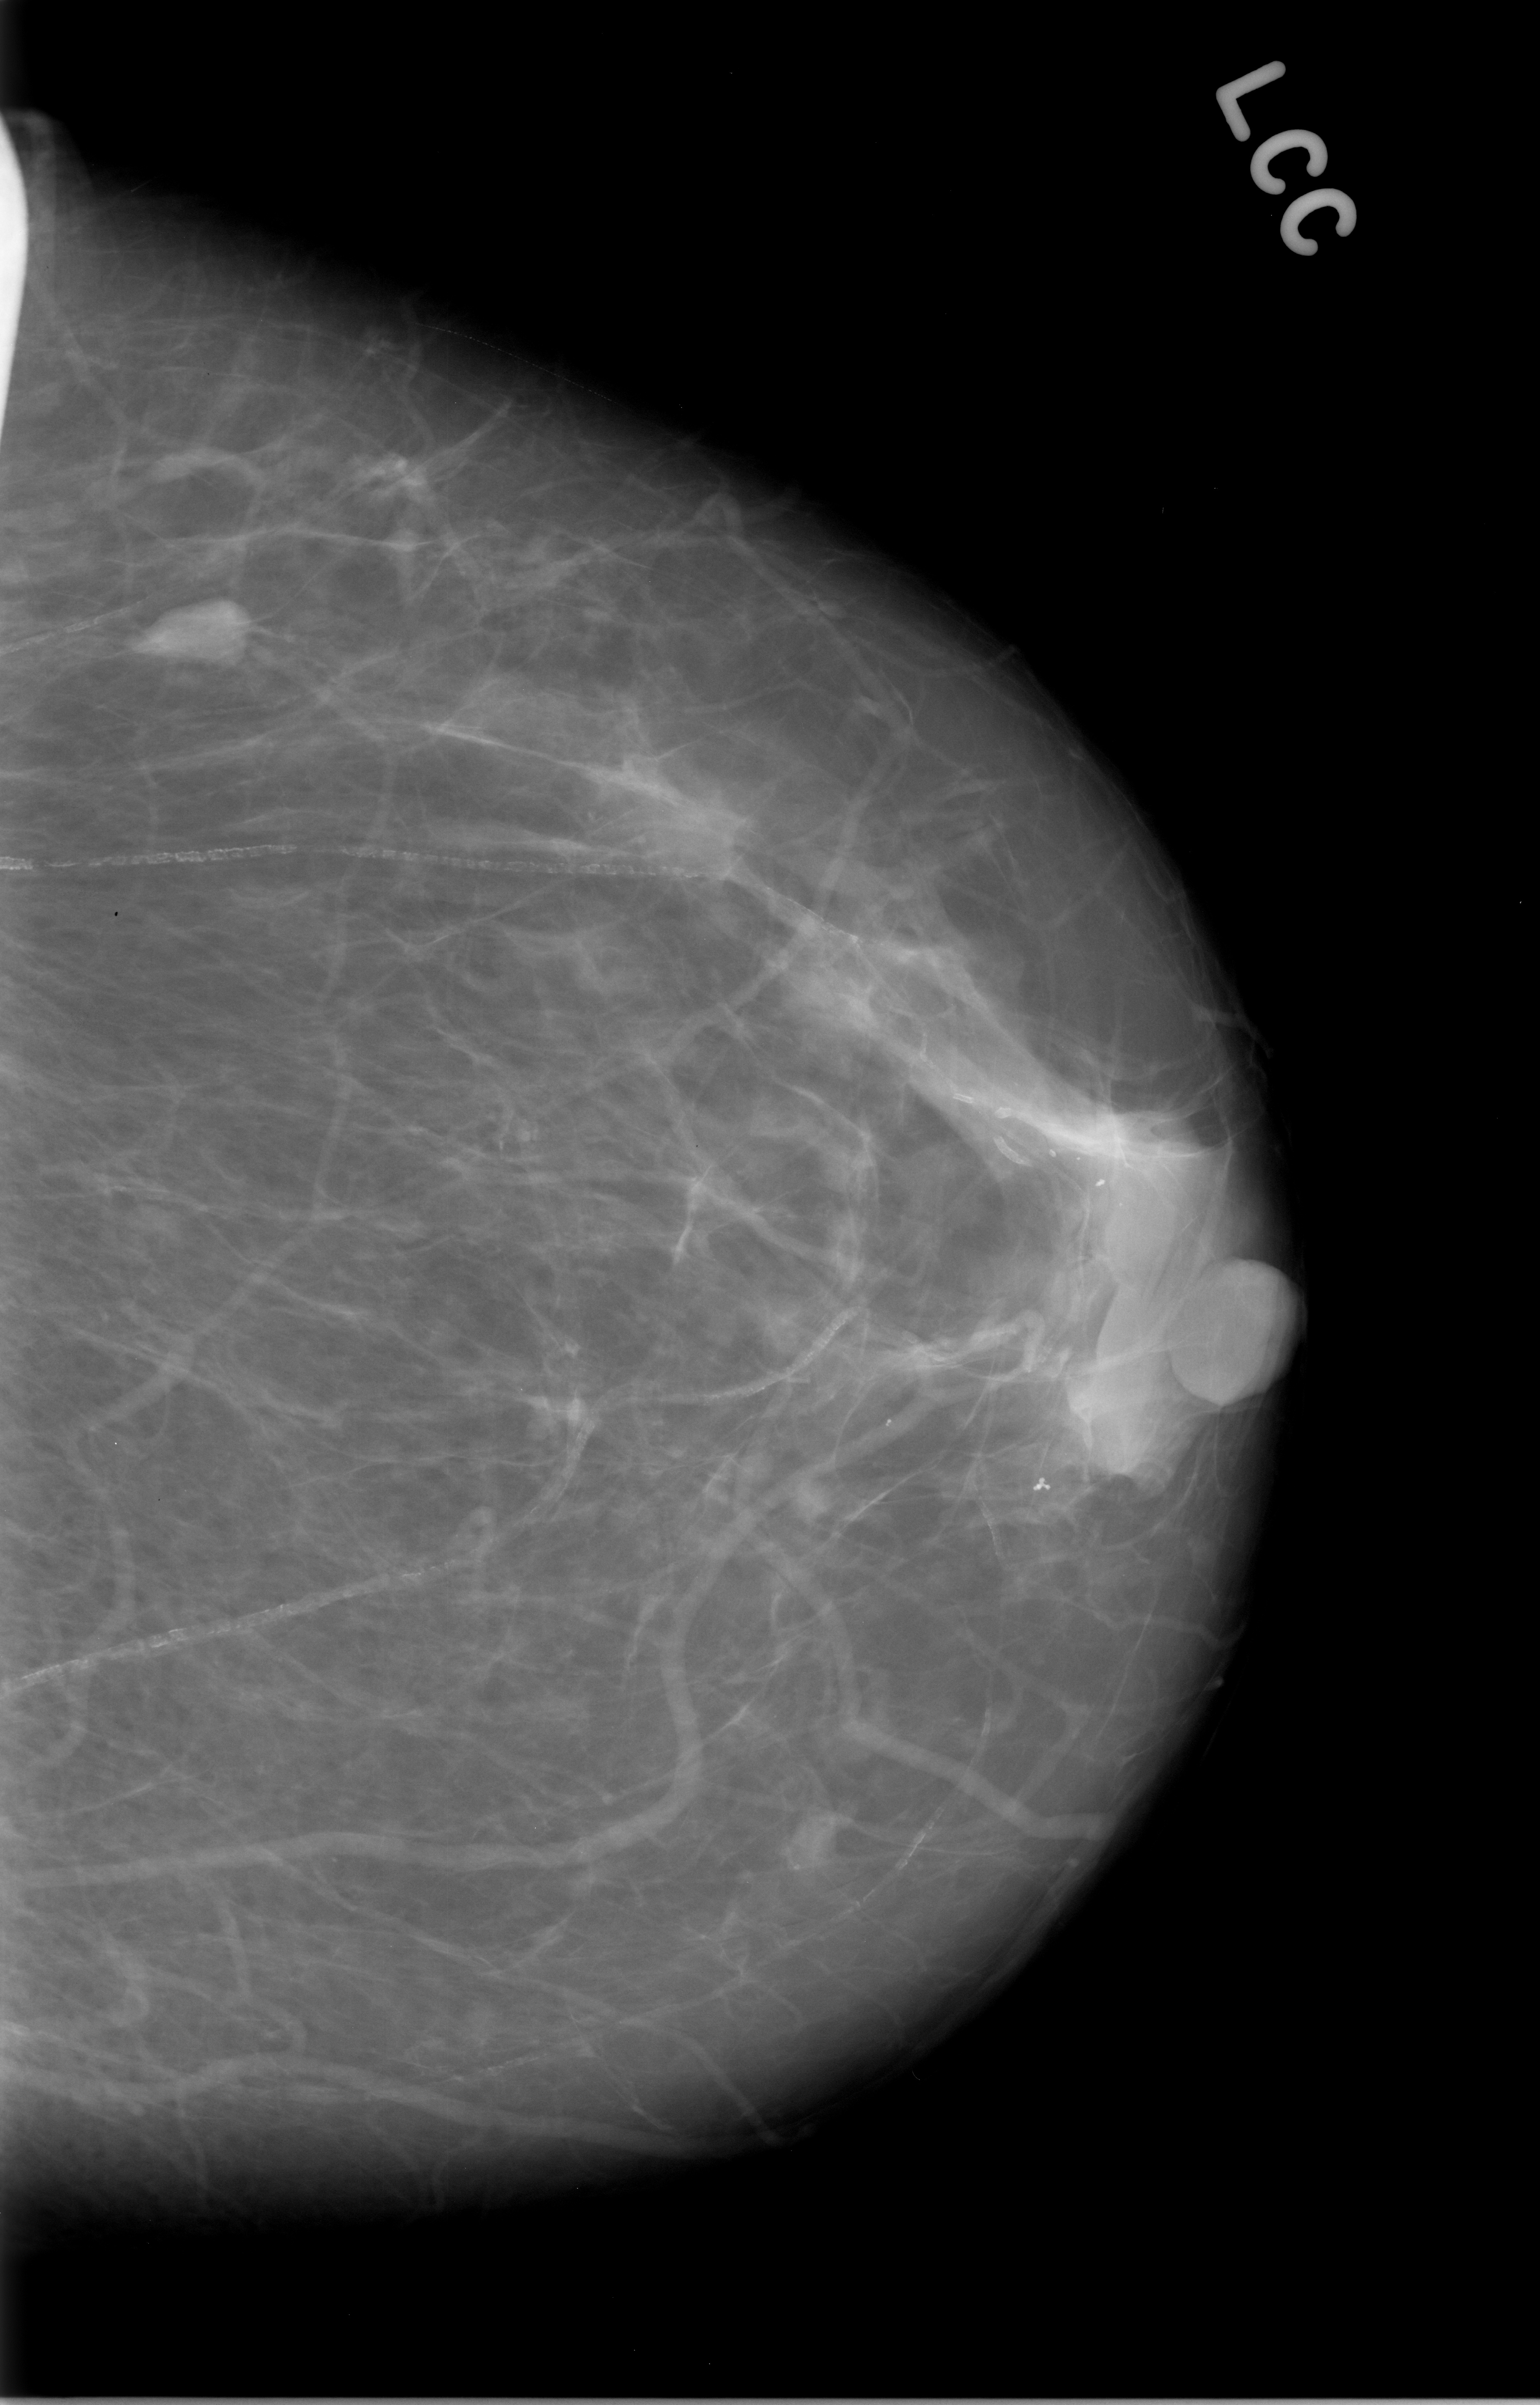
\includegraphics[width=\textwidth]{Figures/completa.jpg}
        \caption{Mama completa}
        \label{completa}
    \end{subfigure}
    \hspace{0.5cm}
    \begin{subfigure}[b]{0.28\textwidth}
        \centering
        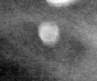
\includegraphics[width=\textwidth]{Figures/cropped.jpg}
        \caption{Recorte da lesão}
        \label{cropped}
    \end{subfigure}
    \hspace{0.5cm}
        \begin{subfigure}[b]{0.28\textwidth}
        \centering
        
\includegraphics[width=\textwidth]{Figures/roi.jpg}
        \caption{Região de interesse}
        \label{roi}
    \end{subfigure}

    \caption{Imagens do conjunto de dados antes da filtragem.}
    \label{banco_dados}
\end{figure}

Para a utilização nesta pesquisa, foi necessário realizar um processo de filtragem e organização do conjunto de dados, de forma a selecionar apenas as imagens da mama completa ao treinamento do modelo gerador. Considerando que o objetivo da rede generativa adversarial (GAN) é aprender padrões visuais globais das mamografias, optou-se pelo uso exclusivo das imagens de mama completa, descartando as versões recortadas e as máscaras de ROI. Todo o processo é executado de forma automatizada por um \textit{script} de construção de manifesto, e os quantitativos por classe e por etapa são registrados em disco para garantir reprodutibilidade.

Para evitar a presença de imagens redundantes, aplicou-se uma etapa de remoção de quase-duplicatas baseada em \textit{hashing} perceptual (\textit{perceptual hash}, pHash) com distância de Hamming: imagens cuja distância era inferior ou igual a um limiar pré-definido foram colapsadas em um único representante, e as duplicatas foram registradas em \textit{log}. Além disso, o identificador de paciente (\textit{patient\_id}), recuperado dos arquivos CSV de casos (massas e calcificações) da CBIS-DDSM, foi mantido em cada registro, possibilitando a separação em nível de paciente descrita na seção seguinte. Após a seleção de imagens de mama completa e a remoção de quase-duplicatas, o conjunto resultou em 553 imagens, sendo 245 classificadas como malignas e 308 como benignas.

Em seguida, o arquivo CSV original foi ajustado, mantendo as colunas essenciais para o treinamento: \textit{patient\_id}, \textit{pathology} e \textit{image file path}, correspondentes ao paciente, à classe da amostra e ao caminho da respectiva imagem. O rótulo binário foi definido pelo mapeamento da coluna \textit{pathology}: amostras \textit{MALIGNANT} foram mapeadas para o rótulo 1 (maligno), enquanto \textit{BENIGN} e \textit{BENIGN\_WITHOUT\_CALLBACK} foram mapeadas para o rótulo 0 (benigno). Essa padronização possibilitou uma distinção clara entre as duas principais classes do estudo: benigno e maligno.

Por fim, todas as imagens foram orientadas na mesma direção, independentemente de representarem a mama esquerda ou direita. Essa normalização foi feita para evitar que o modelo aprendesse padrões relacionados apenas à posição anatômica, concentrando-se nas características visuais e estruturais das lesões. Dessa forma, o conjunto de dados foi devidamente preparado para as etapas subsequentes de pré-processamento, treinamento e avaliação do modelo de geração, garantindo coerência, qualidade e integridade das informações utilizadas.

O conjunto de imagens de mama completa, após a remoção de quase-duplicatas, totalizou 553 imagens (308 benignas e 245 malignas). As 439 imagens reais pertencentes à partição de desenvolvimento (DEV) ficam disponíveis ao treinamento do modelo generativo, uma vez que o desbalanceamento moderado é aceitável para o gerador e os exemplos benignos adicionais são benéficos ao aprendizado da estrutura global da mama. Para o classificador, por outro lado, as classes de DEV são balanceadas por \textit{downsampling} das benignas, resultando em um conjunto real balanceado de 194 amostras por classe (388 imagens no total); o conjunto de teste, mantido bloqueado, é igualmente balanceado, com 49 imagens por classe (98 no total). As imagens benignas removidas pelo balanceamento são excluídas do conjunto real do classificador, mas nunca contaminam o conjunto de teste: como a separação é feita em nível de paciente, nenhuma imagem dessas pacientes migra para o TEST. As contagens exatas por classe e por partição são registradas em arquivo (JSON) para reprodutibilidade.

Algumas limitações foram identificadas referentes ao conjunto de dados. Primeiramente, o número total de imagens é relativamente pequeno para a aplicação de modelos de classificação, o que aumenta o risco de sobreajuste (\textit{overfitting}). Além disso, apesar do equilíbrio relativo entre classes benignas e malignas, o conjunto ainda é limitado em termos de diversidade de casos. Estratégias de aumento da variabilidade, como técnicas de \textit{data augmentation} e geração sintética de imagens, foram adotadas e serão detalhadas nas próximas seções.

\section{Protocolo experimental livre de vazamento de dados}
\label{sec:protocolo}

A concepção experimental deste trabalho foi revista para eliminar uma fonte de vazamento de dados (\textit{data leakage}) presente na versão anterior. Naquela versão, o modelo generativo era treinado uma única vez sobre todas as 553 imagens reais e um único conjunto sintético era concatenado a todas as dobras de treinamento de uma validação cruzada, além de o filtro LPIPS comparar as imagens sintéticas com o conjunto real completo. Como o gerador e o filtro tinham acesso a imagens posteriormente utilizadas na validação, informação do conjunto de avaliação vazava para o treinamento, produzindo estimativas otimistas e inválidas de desempenho.

Para corrigir esse problema, adotou-se como protocolo principal um \textit{hold-out} estratificado em nível de paciente. As 553 imagens são divididas, por paciente (\textit{GroupShuffleSplit} sobre \textit{patient\_id}), em uma partição de desenvolvimento (DEV, aproximadamente 80\%) e um conjunto de teste (TEST, aproximadamente 20\%) mantido bloqueado e utilizado somente na mensuração final. A separação em nível de paciente garante que nenhuma paciente contribua com imagens simultaneamente para DEV e TEST.

Nesse protocolo, o gerador \textit{StyleGAN2-ADA} é treinado exclusivamente com imagens de DEV e o filtro LPIPS referencia apenas as imagens reais de DEV; o conjunto TEST não é acessado por qualquer etapa generativa ou de seleção. O classificador \textit{EfficientNet-B0} é treinado sobre a combinação de imagens reais e sintéticas de DEV, com seleção de modelo e parada antecipada em uma partição de validação interna extraída somente de DEV, e é avaliado sobre o TEST bloqueado. Para cada proporção sintético:real (0:1, 1:1, 2:1, 3:1 e 4:1), todo o treinamento do classificador é repetido por 10 sementes independentes, produzindo uma distribuição de métricas de teste por proporção que viabiliza intervalos de confiança e testes de significância pareados.

Está também disponível uma variante mais rigorosa, baseada em \textit{Stratified GroupKFold} em nível de paciente, na qual o gerador é retreinado a cada dobra apenas com os dados de treino daquela dobra e o filtro LPIPS referencia somente esses dados. Essa variante elimina o vazamento por construção, sendo reservada como referência para reprodução com maior poder computacional. Ambos os protocolos são livres de vazamento e corrigem diretamente a limitação de vazamento de dados apontada na avaliação por pares.

\section{Geração de imagens sintéticas}

\subsection{Arquitetura do modelo de geração}

O desenvolvimento do modelo generativo deste trabalho envolveu a avaliação de diferentes arquiteturas de \textit{Generative Adversarial Networks} (GANs) condicionais, incluindo DCGAN condicional e WGAN-GP condicional. Ambos os modelos foram inicialmente testados como base para a geração de mamografias sintéticas, permitindo observar a capacidade de aprendizado de padrões visuais das classes benignas e malignas. Embora tenham apresentado resultados coerentes em termos de estrutura geral das imagens, ambos demonstraram limitações na fidelidade visual e na preservação de detalhes anatômicos sutis, evidenciando a necessidade de uma arquitetura mais avançada.

Foi desenvolvida uma arquitetura híbrida que combinou elementos da DCGAN condicional e da WGAN-GP condicional, com o objetivo de unir a capacidade de representação convolucional profunda da primeira à estabilidade de treinamento e robustez da segunda. Essa fusão resultou na \textit{Conditional Wasserstein Deep Convolutional GAN with Gradient Penalty} (cWGAN-GP), uma abordagem que emprega convoluções transpostas no gerador e convoluções diretas no discriminador, associadas à função de perda de Wasserstein com penalização de gradiente, que reduz oscilações durante o aprendizado adversarial, representada pela Figura \ref{cwgan}. 

\begin{figure}[H]
    \centering
    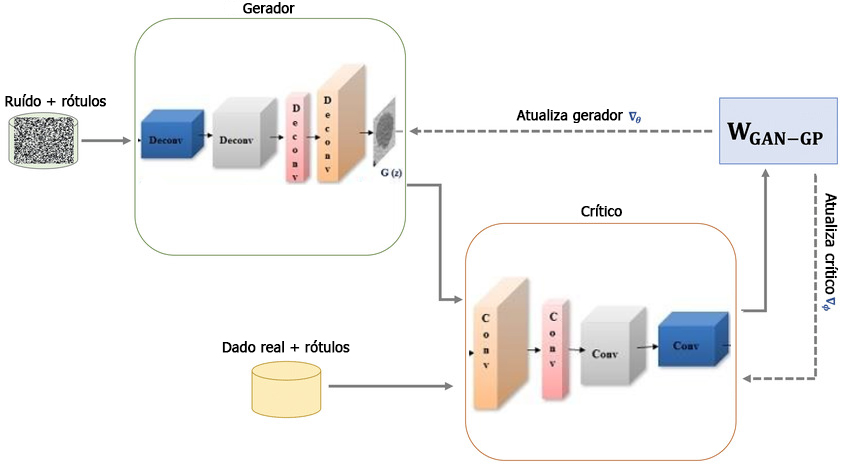
\includegraphics[width=0.95\linewidth]{Figures/cwgan.jpg}
    \caption{Arquitetura da cWGAN-GP}
    \label{cwgan}
\end{figure}

O modelo recebe como entrada um vetor de ruído concatenado a um vetor de rótulo \textit{one-hot}, permitindo controlar a classe de saída (benigno ou maligno). A implementação possibilitou gerar amostras com estrutura anatômica coerente e melhor estabilidade de convergência, embora ainda apresentasse ruídos texturais e imprecisões sutis nas bordas das imagens, como mostra a Figura \ref{mamwgan}, indicando a necessidade de arquiteturas mais avançadas.


\begin{figure}[H]
    \centering
    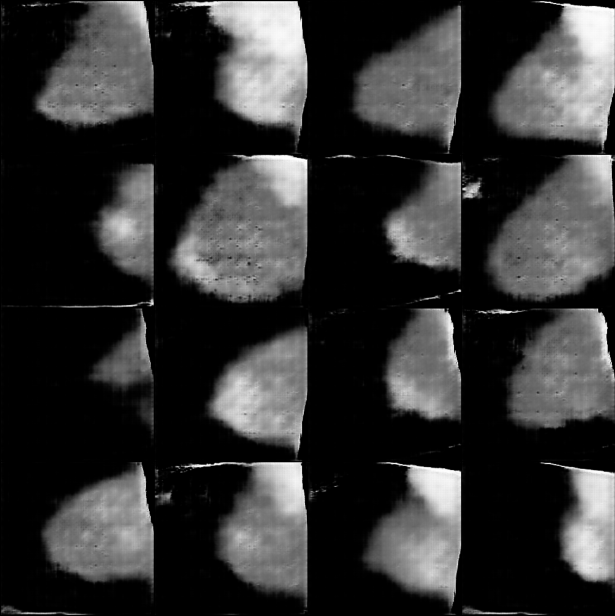
\includegraphics[width=0.6\linewidth]{Figures/mamografiaswgan.png}
    \caption{Mamografias sintéticas geradas pela cWGAN-GP}
    \label{mamwgan}
\end{figure}

Os resultados apresentados na Figura \ref{resultados_lpips_wgan} mostram que a arquitetura cWGAN-GP obteve média de 0.352 e mediana de 0.347 nos valores de LPIPS, indicando uma similaridade perceptual moderada entre as imagens geradas e as reais. Apesar de demonstrar estabilidade na geração, esses valores refletem uma limitação do modelo em capturar com precisão as variações de textura e contraste características das mamografias. 

\begin{figure}[H]
    \centering
    % Subfigura (a)
    \begin{subfigure}[b]{0.45\textwidth}
        \centering
        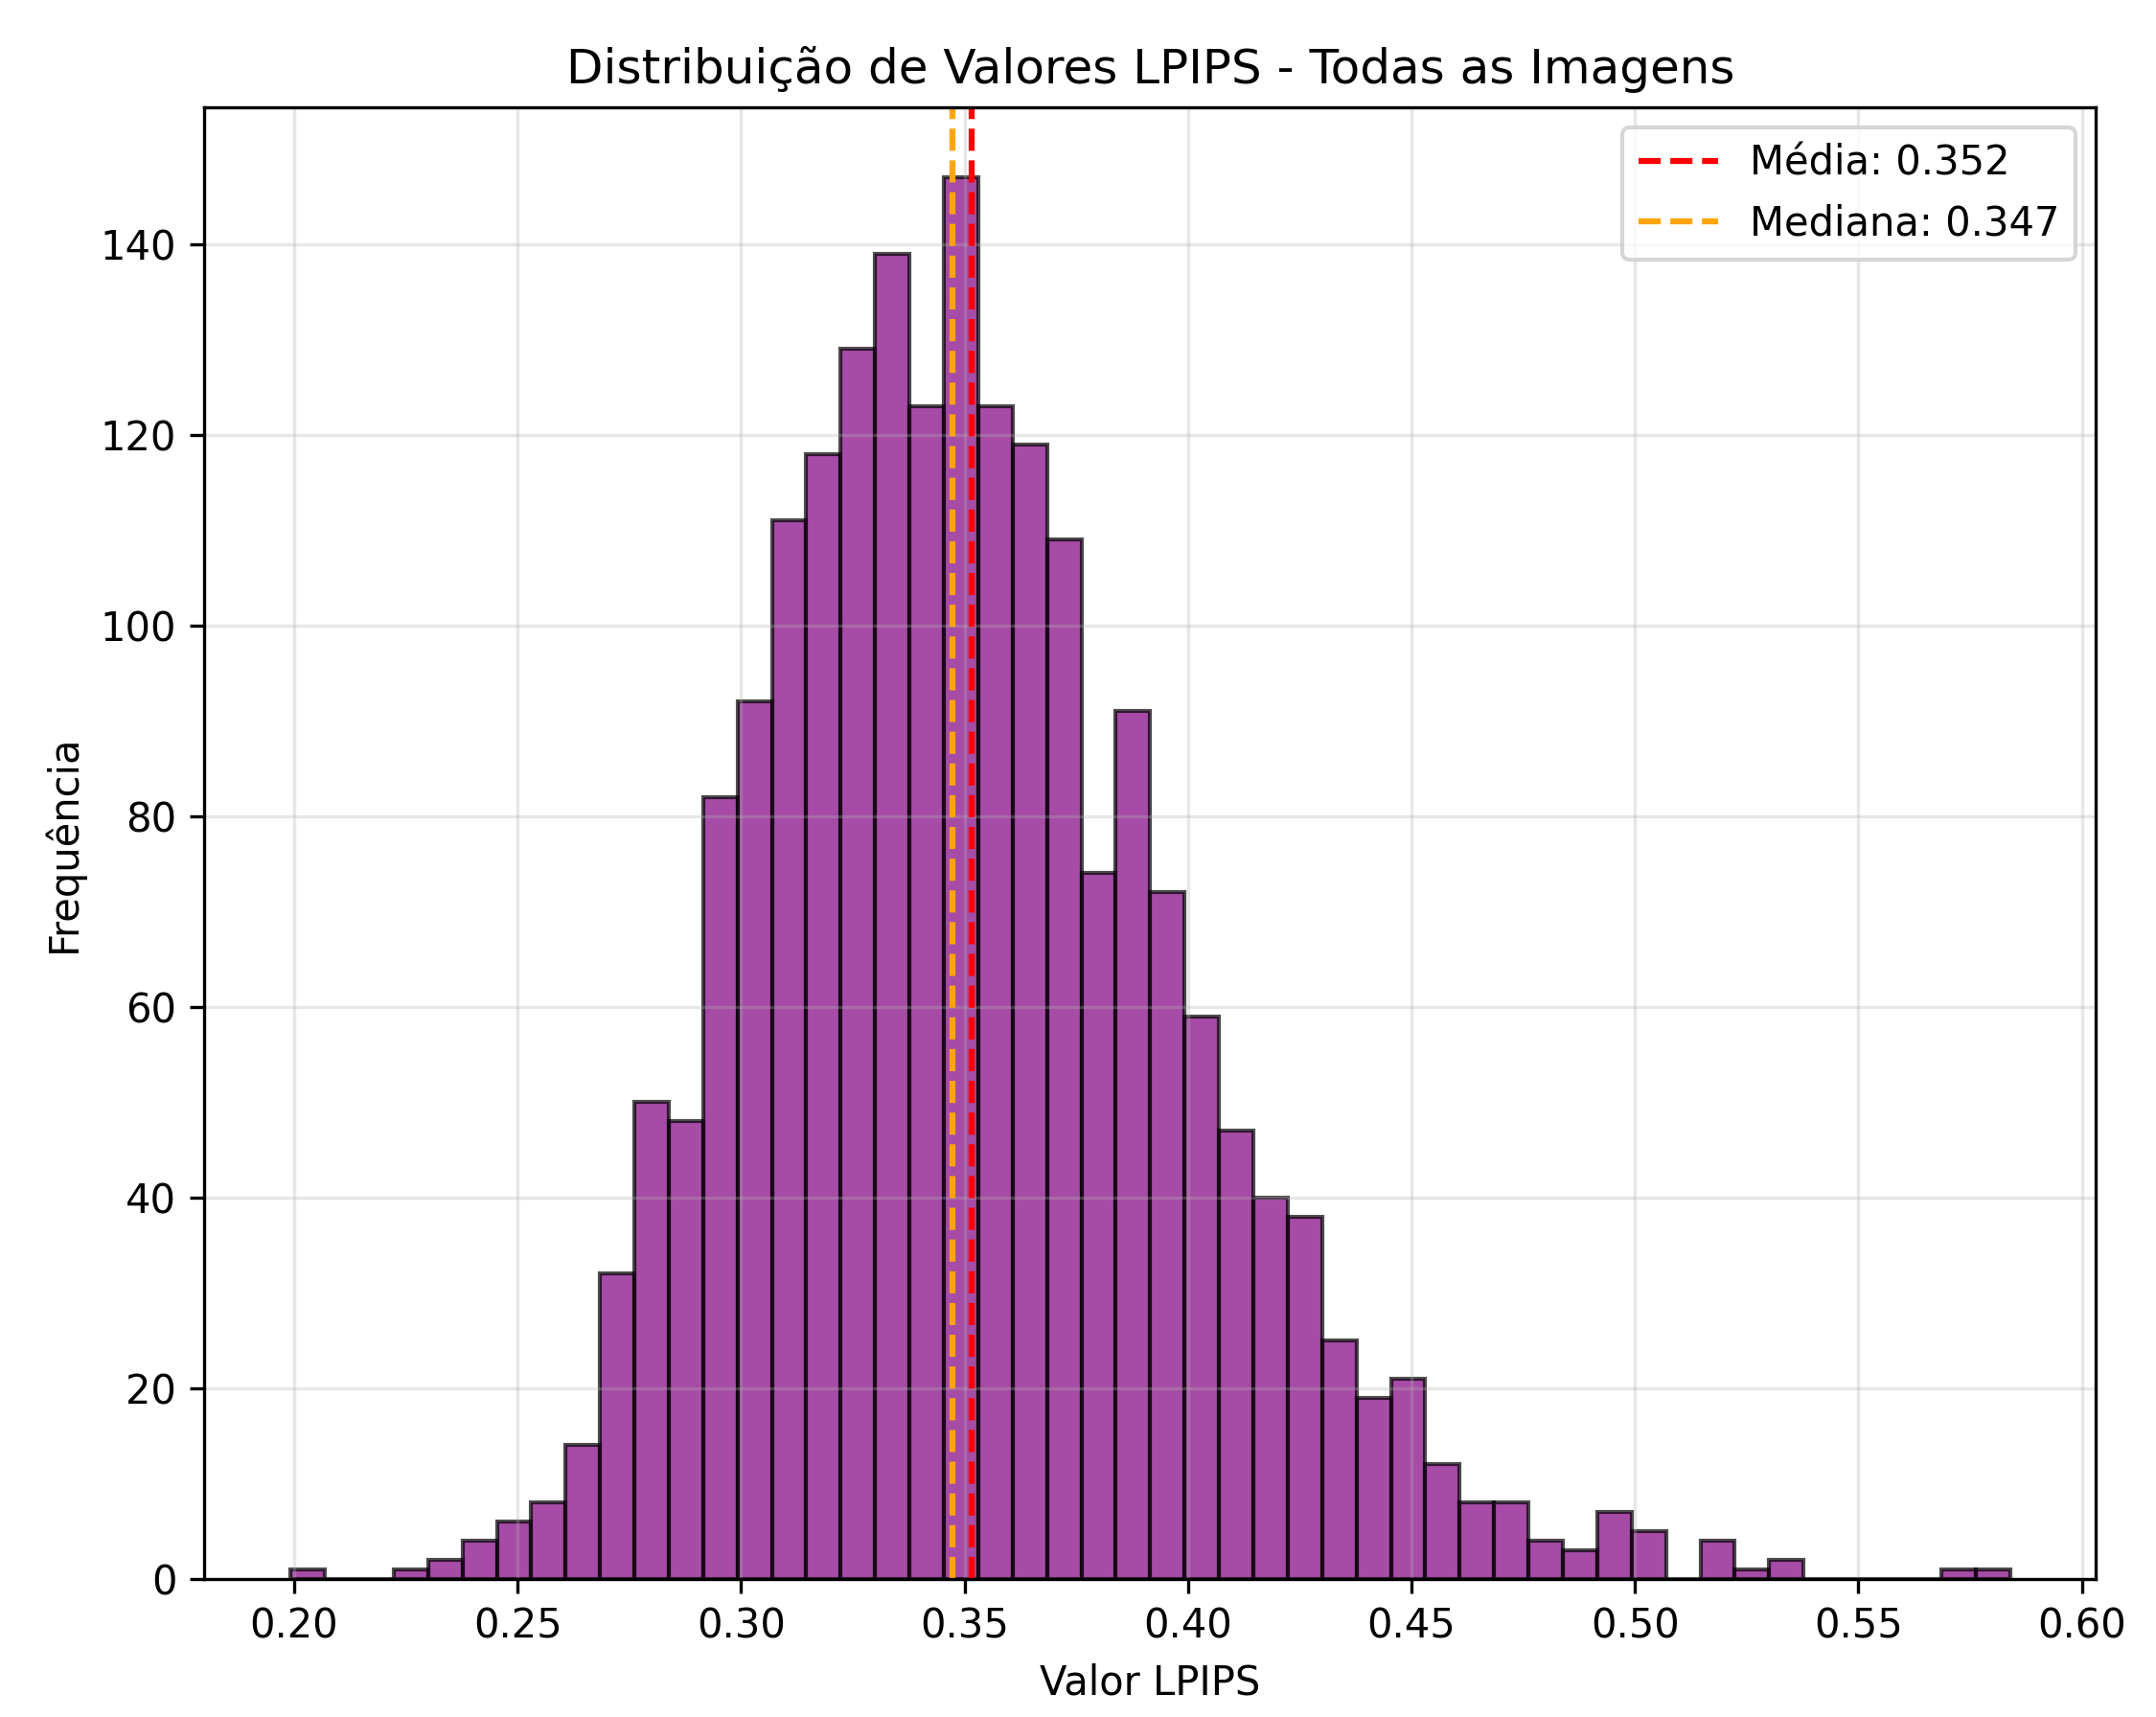
\includegraphics[width=\textwidth]{Figures/wgan_distrib.png}
        \caption{Distribuição LPIPS para todas as imagens}
        \label{distr_lpips_wgan}
    \end{subfigure}
    \hfill
    % Subfigura (b)
    \begin{subfigure}[b]{0.45\textwidth}
        \centering
        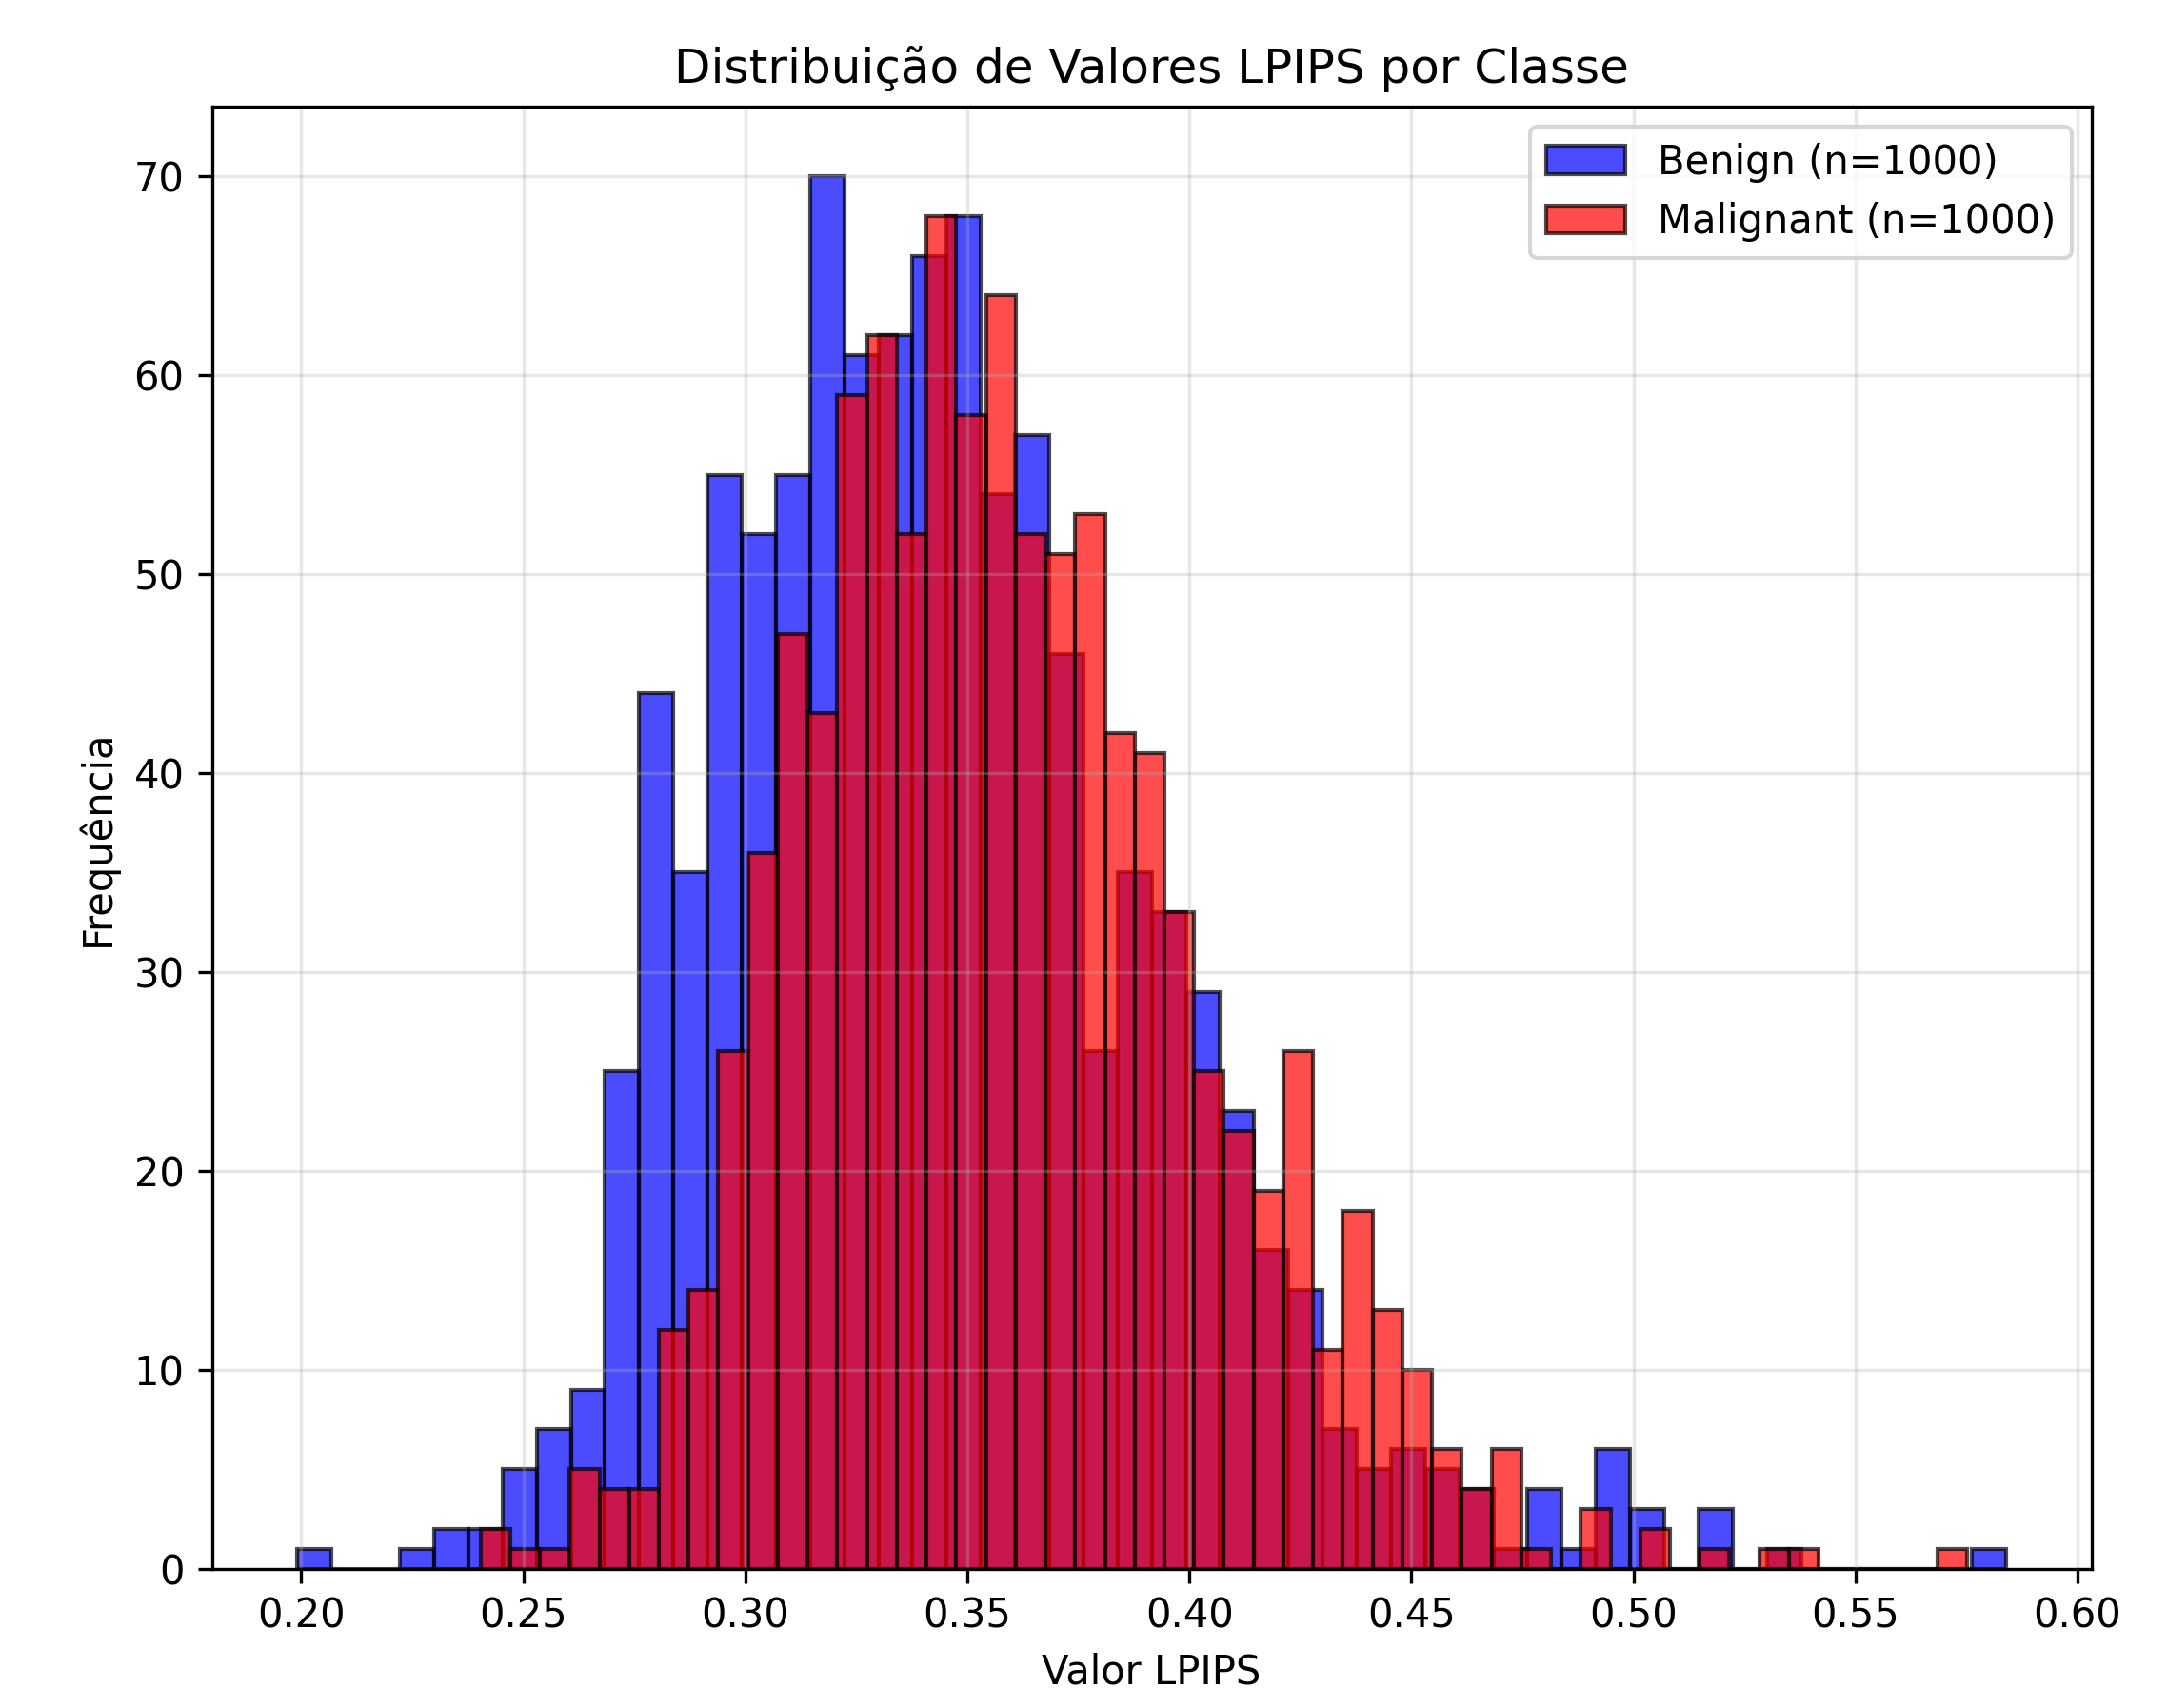
\includegraphics[width=\textwidth]{Figures/wgan_class.png}
        \caption{Distribuição LPIPS para cada classe de imagem}
        \label{distr_class_lpips_wgan}
    \end{subfigure}
    % Subfigura (c)
    \begin{subfigure}[b]{0.45\textwidth}
        \centering
        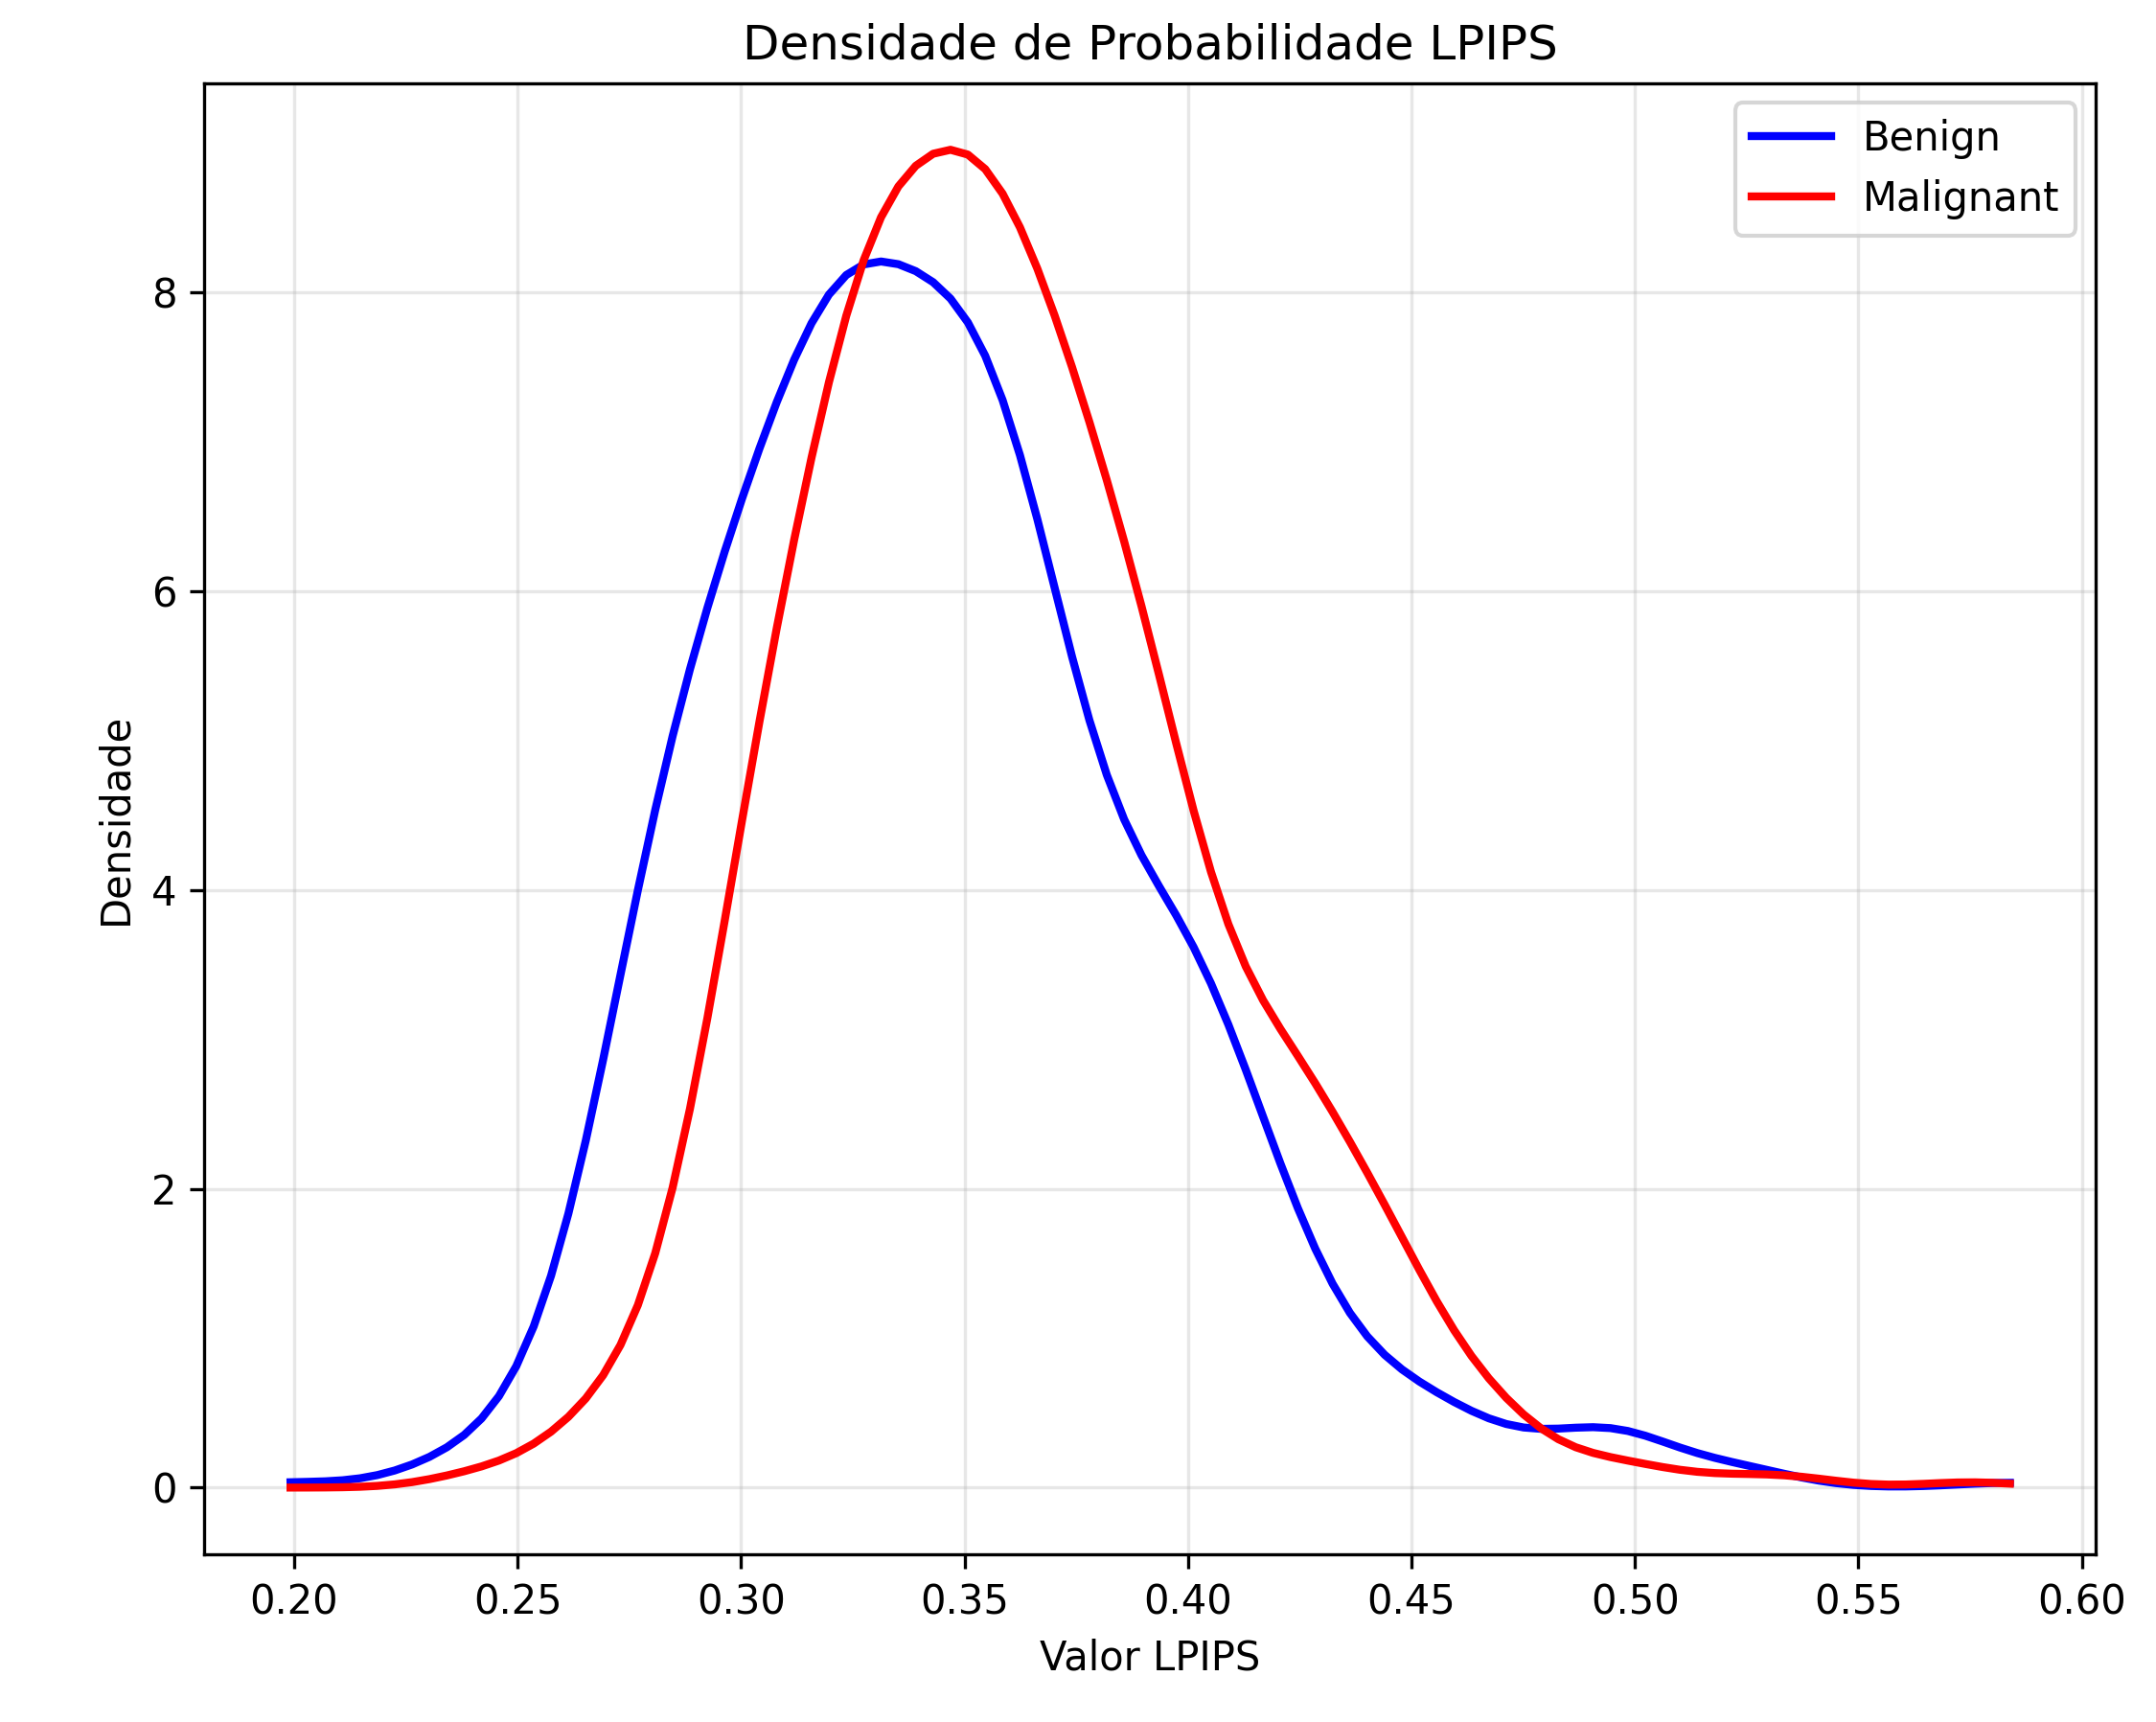
\includegraphics[width=\textwidth]{Figures/wgan_dens.png}
        \caption{Densidade LPIPS}
        \label{dens_lpips_wgan}
    \end{subfigure}
    \hfill
    % Subfigura (d)
    \begin{subfigure}[b]{0.45\textwidth}
        \centering
        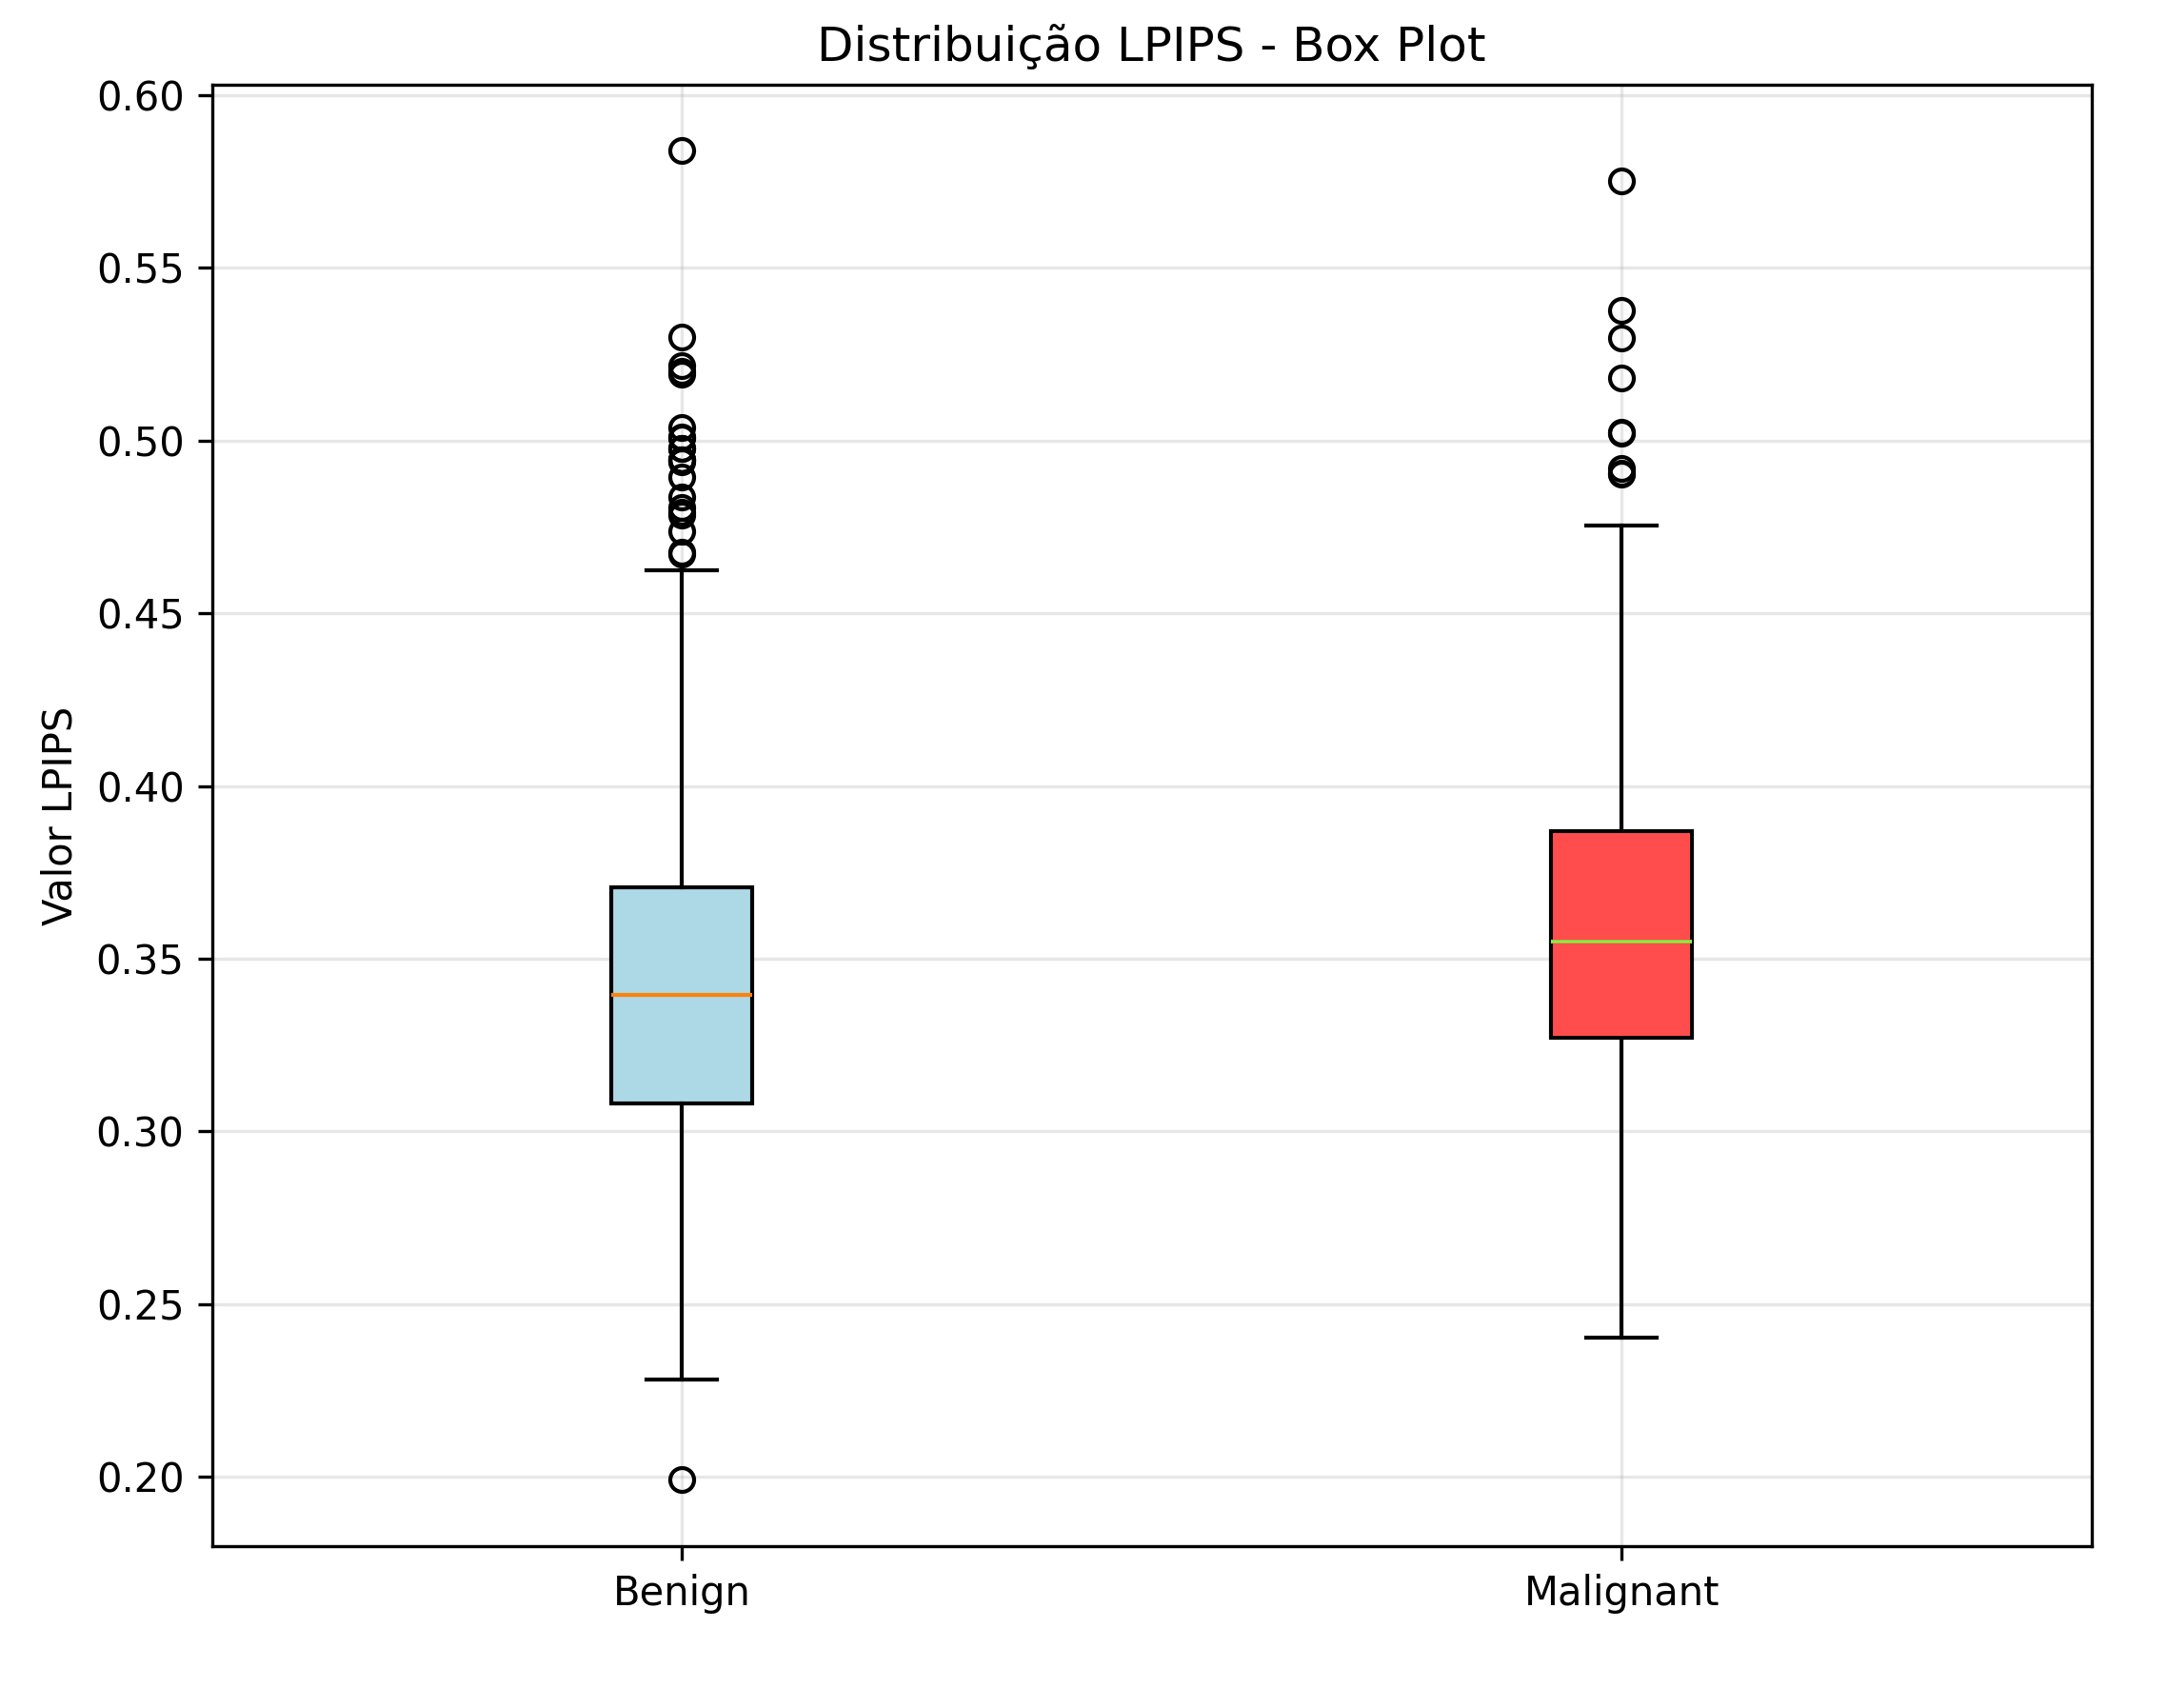
\includegraphics[width=\textwidth]{Figures/wgan_boxplot.png}
        \caption{Box plot LPIPS}
        \label{box_lpips_wgan}
    \end{subfigure}

    \caption{Gráficos dos valores do LPIPS na geração de 1000 imagens para cada classe usando WGAN-GP. Em laranja estão representadas as classes malignas e em azul as benignas.}
    \label{resultados_lpips_wgan}
\end{figure}


Considerando essas limitações e o objetivo de aprimorar a qualidade perceptual das imagens, optou-se pela adoção do \textit{StyleGAN2-ADA} condicional \cite{karras2020ada}. Essa escolha foi motivada pela capacidade do \textit{StyleGAN2-ADA} de representar detalhes morfológicos complexos com maior realismo, aliando a abordagem \textit{style-based} à técnica de \textit{Adaptive Discriminator Augmentation} (ADA), o que possibilita um treinamento estável mesmo com conjuntos de dados limitados. Assim, a nova arquitetura busca superar as restrições observadas no cWGAN-GP, produzindo imagens de mamografia com maior fidelidade perceptual e melhor separabilidade entre as classes.

O gerador condicional do \textit{StyleGAN2-ADA}, ilustrado na Figura~\ref{gerador}, recebe um vetor latente combinado à condição da classe e o transforma progressivamente em uma imagem sintetizada por meio de blocos de convolução baseados em \textit{style modulation}. Essa abordagem permite controlar características de alto e baixo nível durante o processo de geração, conferindo maior precisão na representação de estruturas morfológicas presentes em mamografias.
\begin{figure}[H]
    \centering
    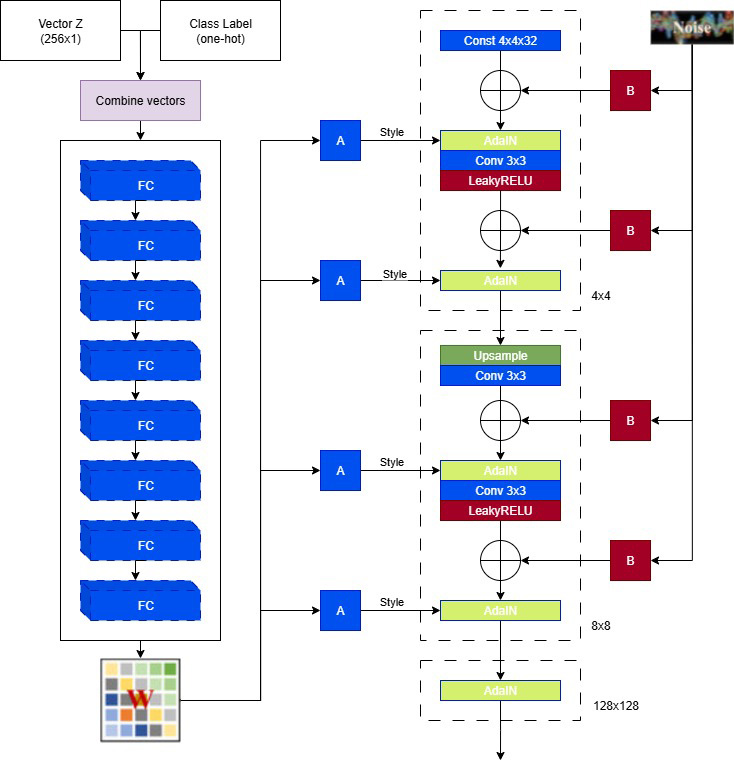
\includegraphics[width=0.95\linewidth]{Figures/generator.jpg}
    \caption{Arquitetura do gerador}
    \label{gerador}
\end{figure}

O discriminador condicional, por sua vez, recebe a imagem gerada concatenada à condição da classe e aplica uma sequência de blocos convolucionais com ativação Leaky ReLU, integrando os princípios de R1 regularization e ADA para melhorar a estabilidade e evitar sobreajuste (\textit{overfitting}), Figura \ref{discriminador}. Durante o treinamento, a arquitetura permite que o gerador aprenda características detalhadas das mamografias, enquanto o discriminador fornece \textit{feedback} contínuo sobre realismo e consistência com a classe fornecida.

\begin{figure}[H]
    \centering
    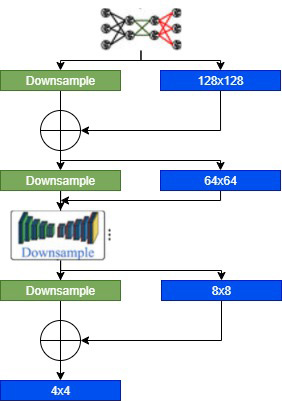
\includegraphics[width=0.4\linewidth]{Figures/discriminator.jpg}
    \caption{Arquitetura do discriminador}
    \label{discriminador}
\end{figure}

O modelo StyleGAN2-ADA condicional demonstrou superioridade em comparação às arquiteturas previamente testadas, produzindo imagens sintéticas de alta qualidade, com melhor preservação de texturas e estruturas anatômicas críticas. A concatenação das informações de classe ao vetor latente possibilitou um controle mais preciso sobre o conteúdo gerado, garantindo que o modelo reproduzisse características específicas de mamografias benignas e malignas. Essa abordagem consolidou o StyleGAN2-ADA condicional como a arquitetura escolhida para a síntese de imagens neste estudo, estabelecendo uma base sólida para futuras etapas de aumento de dados e treinamento de modelos de classificação.
    
\subsection{Pré-processamento de imagens}

Para garantir que as mamografias estivessem em um formato adequado ao treinamento do modelo \textit{StyleGAN2-ADA} condicional, todas as imagens foram primeiramente convertidas para escala de cinza, resultando em um único canal de entrada. Em seguida, as imagens foram redimensionadas para $128 \times 128$ pixels utilizando interpolação bilinear. Essa resolução inicial foi escolhida como um compromisso entre a qualidade visual das imagens e a limitação de memória da GPU, permitindo o treinamento com lotes (\textit{batch size}) de 8 imagens.

Os valores dos pixels foram então convertidos em tensores do PyTorch e normalizados para o intervalo $[-1, 1]$, o que é compatível com as funções de ativação Leaky ReLU empregadas nas redes do gerador e do discriminador. Cada imagem recebeu um rótulo binário indicando se a amostra era benigna (0) ou maligna (1), com base nas informações presentes no arquivo CSV de metadados. Esses rótulos foram posteriormente convertidos em vetores \textit{one-hot} de dimensão 2, permitindo que o gerador criasse imagens condicionadas à classe correspondente.

Durante o treinamento, aplicou-se uma estratégia de aumento de dados adaptativa (\textit{Adaptive Discriminator Augmentation, ADA}) para aumentar a diversidade das imagens e reduzir o sobreajuste. As transformações utilizadas incluíram \textit{flip} horizontal com probabilidade de 50\% e pequenas rotações de até 5°. A probabilidade de aplicação do ADA foi ajustada dinamicamente em função do desempenho do discriminador, visando uma meta de 60\%.

O pré-processamento também considerou a preparação eficiente para a GPU, com carregamento de dados em lotes de 8 imagens, utilizando duas \textit{threads} e memória pinada quando disponível. Em conformidade com o protocolo livre de vazamento (Seção~\ref{sec:protocolo}), o treinamento do gerador utilizou exclusivamente as imagens da partição de desenvolvimento (DEV), organizadas de maneira a manter uniformidade na entrada da rede.
    
\subsection{Treinamento do modelo de geração}

O modelo do gerador foi inicializado com pesos distribuídos normalmente ($\mu = ~0.\\ \sigma = 1$), enquanto o discriminador recebeu configuração similar. O vetor latente $z \in \mathbb{R}^{256}$ foi combinado com os vetores \textit{one-hot} das classes (benigno ou maligno) para formar a entrada condicionada do gerador. A rede mapeadora (\textit{Mapping Network}) processou $z$ para gerar o vetor $A \in \mathbb{R}^{256}$, que modulou as camadas do gerador através de \textit{Adaptive Instance Normalization} (AdaIN). Cada bloco do gerador aplicou convoluções, ruído estocástico e funções de ativação Leaky ReLU, permitindo a síntese progressiva de imagens de maior resolução.

O treinamento seguiu o esquema de otimização adversarial com \textit{Adam} para o gerador e o discriminador, usando taxas de aprendizado de $0.0025$ e parâmetros $\beta_1 = 0.0$ e $\beta_2 = 0.99$. As funções de perda empregadas foram a \textit{logistic loss} para ambos os modelos e a penalidade R1 aplicada ao discriminador a cada 32 iterações. Além disso, o treinamento utilizou precisão mista (\textit{automatic mixed precision}) para reduzir consumo de memória e acelerar o processamento.

O modelo também incorporou a estratégia de aumento de dados adaptativa (\textit{ADA}), ajustando dinamicamente a probabilidade de aplicar transformações como \textit{flip} horizontal e rotações pequenas, visando manter uma meta de $60\%$ de eficácia no discriminador. Para monitoramento, \textit{checkpoints} foram salvos, incluindo pesos do gerador e discriminador, otimizadores e histórico das perdas, enquanto amostras geradas fixas eram armazenadas para visualização da evolução do treinamento.\\

O treinamento foi conduzido por 400 épocas, com cada época percorrendo todo o \textit{dataset}, garantindo que tanto o gerador quanto o discriminador fossem atualizados em todas as iterações. Essa configuração permitiu que o gerador aprendesse a produzir imagens médicas de alta fidelidade condicionadas à classe, minimizando sobreajuste e mantendo diversidade visual.

\subsection{Uso do LPIPS para avaliação de qualidade das imagens geradas}

Diversas métricas foram avaliadas na literatura para mensurar a qualidade de imagens geradas por redes neurais, dentre as quais destacam-se o PSNR (\textit{Peak Signal-to-Noise Ratio}), o SSIM (\textit{Structural Similarity Index}) e o LPIPS (\textit{Learned Perceptual Image Patch Similarity}). Enquanto o PSNR e o SSIM baseiam-se em diferenças de intensidade e estrutura de pixels, o LPIPS utiliza representações extraídas de redes neurais profundas, permitindo uma avaliação perceptual mais próxima da visão humana.

Pawar et al. \cite{pawar2024esm} mostraram que modelos de geração de imagens com aparência mais realista, como o SRGAN, obtiveram baixos valores de PSNR e SSIM, mas se destacaram significativamente em LPIPS. Isso indica que as métricas tradicionais nem sempre refletem a qualidade visual percebida, especialmente quando o objetivo é gerar dados sintéticos visualmente convincentes.

Dessa forma, neste trabalho optou-se pelo uso do LPIPS como métrica principal de avaliação, por apresentar maior correlação com a percepção humana e melhor sensibilidade a diferenças perceptuais sutis, mostrando-se, portanto, adequado para mensurar a fidelidade visual e o realismo das imagens sintéticas geradas. A aplicação dessa métrica permitiu avaliar a qualidade perceptual das mamografias produzidas em comparação com as imagens reais, conforme ilustrado na Figura \ref{imagens_reais_sinteticas_ben}, que apresenta amostras benignas, e na Figura \ref{imagens_reais_sinteticas_mal}, que exibe amostras malignas, em ambos os casos, a imagem (a) corresponde à amostra real e a imagem (b) à amostra sintética.

\begin{figure}[H]
    \centering
    % Subfigura (a)
    \begin{subfigure}[b]{0.45\textwidth}
        \centering
        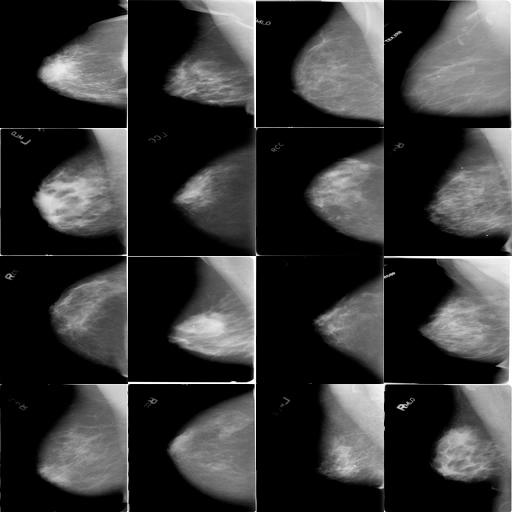
\includegraphics[width=\textwidth]{Figures/ben_real.jpg}
        \caption{Imagem real}
        \label{ben_a}
    \end{subfigure}
    \hfill
    % Subfigura (b)
    \begin{subfigure}[b]{0.45\textwidth}
        \centering
        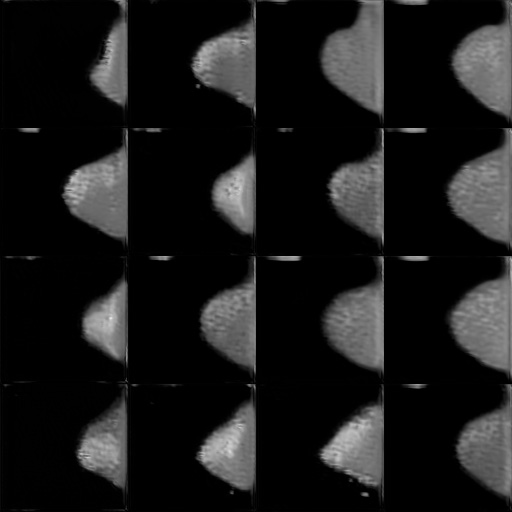
\includegraphics[width=\textwidth]{Figures/ben_sint.jpg}
        \caption{Imagem sintética}
        \label{ben_b}
    \end{subfigure}

    \caption{Mamografias benignas: (a) real e (b) sintética.}
    \label{imagens_reais_sinteticas_ben}
\end{figure}

\begin{figure}[H]
    \centering
    % Subfigura (a)
    \begin{subfigure}[b]{0.45\textwidth}
        \centering
        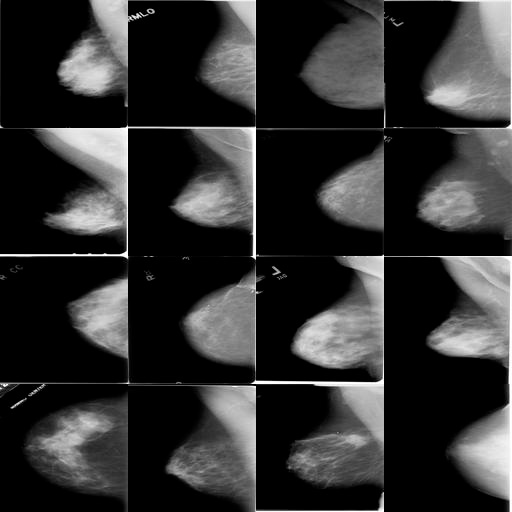
\includegraphics[width=\textwidth]{Figures/mal_real.jpg}
        \caption{Imagem real}
        \label{mal_a}
    \end{subfigure}
    \hfill
    % Subfigura (b)
    \begin{subfigure}[b]{0.45\textwidth}
        \centering
        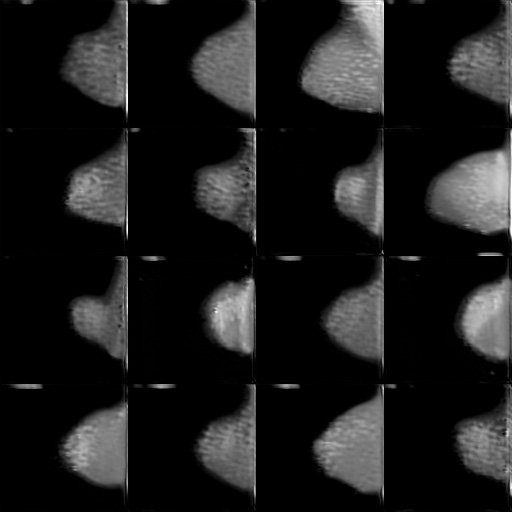
\includegraphics[width=\textwidth]{Figures/mal_sint.jpg}
        \caption{Imagem sintética}
        \label{mal_b}
    \end{subfigure}

    \caption{Mamografias malignas: (a) real e (b) sintética.}
    \label{imagens_reais_sinteticas_mal}
\end{figure}

Para compor o conjunto de dados sintéticos, cada imagem gerada foi caracterizada pela menor distância LPIPS em relação às imagens reais de mesma classe pertencentes ao conjunto DEV. Em vez de fixar arbitrariamente um limiar, realizou-se uma varredura de limiares $\tau \in \{0{,}1;\ 0{,}15;\ 0{,}2;\ 0{,}25;\ 0{,}3\}$, avaliando-se o desempenho no conjunto de teste em função de $\tau$ e o compromisso entre fidelidade e diversidade: valores muito baixos de $\tau$ favorecem a memorização, isto é, a produção de cópias quase idênticas às imagens de treino, enquanto valores muito altos admitem amostras de baixa fidelidade. Conforme detalhado no capítulo de resultados, o valor $\tau = 0{,}2$ do trabalho original mostrou-se inviável sob o protocolo livre de vazamento, por eliminar por completo a retenção de amostras da classe maligna; adotou-se, portanto, $\tau = 0{,}25$ como ponto de operação. Adicionalmente, para as imagens sintéticas retidas realizou-se uma verificação de memorização: computou-se o vizinho real mais próximo (por LPIPS e por distância L2 de pixels) e sinalizaram-se as amostras cuja distância era inferior a um limiar de memorização, reportando-se sua contagem e distribuição. Como o LPIPS, isoladamente, não é capaz de detectar baixa diversidade, essa análise foi complementada pelas métricas FID e KID, reportadas no capítulo de resultados.

As imagens que atenderam a esse critério foram então utilizadas no treinamento da rede EfficientNet-B0, com o objetivo de aumentar a diversidade do conjunto de dados e melhorar a capacidade de generalização do modelo, sem comprometer a qualidade perceptual das amostras utilizadas.

\section{Modelo de classificação}

\subsection{Arquitetura do modelo}

Para a tarefa de classificação de mamografias, foi utilizada a \textit{EfficientNet-B0} \cite{tan2019efficientnet}. Optou-se pela utilização desse modelo, devido ao seu melhor equilíbrio entre acurácia, eficiência computacional e capacidade de generalização.

O modelo foi inicializado com pesos pré-treinados no conjunto de dados \textit{ImageNet}, permitindo o aproveitamento de representações visuais previamente aprendidas. A camada final da rede (\textit{classifier}) foi substituída por uma camada totalmente conectada com um único neurônio de saída e função de ativação sigmoide implícita, adequada para a classificação binária entre amostras benignas e malignas. No modelo reportado, todos os parâmetros da rede, incluindo a base convolucional (\textit{features}), foram ajustados durante o treinamento (\textit{fine-tuning}), de modo a adaptar as representações ao domínio das mamografias. Uma variante com a base convolucional congelada, treinando apenas a camada de classificação, foi avaliada como ablação e apresentou desempenho próximo ao acaso (AUC $\approx 0{,}545$), evidenciando que um classificador funcional, com a base destravada, é necessário para mensurar o efeito das imagens sintéticas.

As imagens de entrada foram redimensionadas para $128 \times 128$ pixels e normalizadas de acordo com as médias e desvios padrão utilizados no treinamento do \textit{ImageNet}. A rede foi treinada utilizando o otimizador \textit{Adam}, com taxa de aprendizado inicial de $1 \times 10^{-4}$ e função de perda binária \textit{Binary Cross-Entropy with Logits (BCEWithLogitsLoss)}. Conforme o protocolo livre de vazamento (Seção~\ref{sec:protocolo}), o modelo foi treinado sobre o conjunto DEV, com seleção de modelo em uma validação interna, e avaliado sobre o conjunto de teste bloqueado, repetindo-se o treinamento por múltiplas sementes.

A escolha da \textit{EfficientNet-B0} mostrou-se adequada por apresentar maior estabilidade durante o treinamento e resultados superiores nas métricas de acurácia, F1-Score e AUC. Além disso, a arquitetura é otimizada para eficiência em GPUs modernas, permitindo melhor aproveitamento dos recursos computacionais sem comprometer a qualidade da classificação das imagens mamográficas.

\subsection{Seleção das imagens sintéticas para o modelo de classificação}

Após o treinamento do modelo de geração, foi realizado um processo de seleção das imagens sintéticas a serem utilizadas no treinamento do modelo de classificação. O objetivo dessa etapa foi garantir que apenas amostras sintéticas com alta qualidade perceptual e diversidade fossem incluídas, reduzindo o risco de introduzir artefatos ou imagens redundantes no conjunto de dados.

Para isso, utilizou-se o LPIPS, cujo cálculo foi feito entre cada imagem sintética gerada e as imagens reais de mesma classe (benigna ou maligna) pertencentes exclusivamente ao conjunto DEV, evitando qualquer referência a imagens do conjunto de teste.

Cada imagem gerada foi comparada com as amostras reais de DEV, e o valor mínimo de LPIPS obtido foi utilizado como medida de similaridade. O limiar de seleção não foi fixado a priori: conforme descrito anteriormente, ele resulta de uma varredura de limiares ($\tau \in \{0{,}1;\ 0{,}15;\ 0{,}2;\ 0{,}25;\ 0{,}3\}$) que equilibra fidelidade e diversidade, adotando-se $\tau = 0{,}25$ como ponto de operação, uma vez que $\tau = 0{,}2$ eliminava por completo a retenção de amostras malignas sob o protocolo livre de vazamento. Uma verificação de vizinho mais próximo foi aplicada para sinalizar e contabilizar eventuais cópias quase idênticas às imagens reais, mitigando o risco de memorização.

As imagens que atenderam ao critério foram salvas em diretórios separados por classe e posteriormente integradas ao conjunto real durante o treinamento supervisionado do classificador. Esse procedimento permitiu aumentar o volume de dados de forma controlada, mantendo a coerência estatística entre os domínios real e sintético.

\subsection{Divisão entre dados reais e sintéticos}

Após a geração das imagens sintéticas pelo modelo \textit{StyleGAN2-ADA}, foi realizada a definição das proporções entre dados reais e sintéticos que seriam utilizadas no treinamento do classificador \textit{EfficientNet-B0}. O objetivo dessa etapa foi investigar o impacto da incorporação de imagens artificiais no desempenho do modelo de classificação, buscando um equilíbrio entre a diversidade introduzida pelos dados gerados e a fidelidade das amostras reais.

Para isso, diferentes proporções de dados foram consideradas, variando desde o uso exclusivo de imagens reais até combinações em que o número de amostras sintéticas superava o de amostras reais. As razões testadas incluíram 1:1, 2:1, 3:1 e 4:1 entre imagens sintéticas e reais, mantendo o mesmo número total de amostras por classe em cada configuração. As imagens sintéticas foram incorporadas apenas ao conjunto de desenvolvimento (DEV); o conjunto de teste (TEST) permaneceu bloqueado e composto exclusivamente por imagens reais, mantendo-se o balanceamento entre as classes benigna e maligna em todas as partições.

A etapa de divisão entre dados reais e sintéticos teve papel definindo a base comparativa para a análise do impacto do uso de dados gerados artificialmente no desempenho da rede \textit{EfficientNet-B0}.

\subsection{Pré-processamento de imagens reais e sintéticas}

Antes do treinamento do modelo de classificação \textit{EfficientNet-B0}, foi necessário realizar o pré-processamento das imagens reais e sintéticas de modo a garantir compatibilidade com a arquitetura e consistência entre as amostras. Todas as imagens foram redimensionadas para $128 \times 128$ pixels, mantendo a resolução utilizada na etapa de geração de imagens sintéticas, o que favoreceu a padronização do fluxo de dados entre os modelos. Diferentemente do modelo gerador, as imagens foram convertidas para o formato RGB, totalizando três canais de entrada, conforme exigido pelos pesos pré-treinados no conjunto \textit{ImageNet}.

As transformações de pré-processamento incluíram a normalização dos valores de pixel utilizando a média $[0.485, 0.456, 0.406]$ e o desvio padrão $[0.229, 0.224, 0.225]$, parâmetros padrão do \textit{ImageNet}. Essa normalização foi fundamental para estabilizar o treinamento e manter a coerência estatística entre o domínio original e o domínio médico das mamografias. Durante o treinamento, foram aplicadas técnicas de aumento de dados (\textit{data augmentation}) com o objetivo de reduzir o sobreajuste (\textit{overfitting}) e aumentar a robustez do modelo frente à variação visual. Entre as transformações aplicadas, destacam-se o \textit{flip} horizontal aleatório e rotações de até 5°, aplicadas de forma independente a cada amostra.

A etapa de carregamento das imagens foi implementada com o \textit{DataLoader} do PyTorch, utilizando lotes de 32 amostras e duas threads para leitura paralela de dados. Sempre que disponível, foi empregada a memória pinada para otimizar a transferência entre CPU e GPU. Esse procedimento garantiu maior eficiência no treinamento, aproveitando os recursos da GPU.

Por fim, as imagens foram organizadas em estruturas balanceadas de classes, correspondentes aos rótulos binários 0 (benigna) e 1 (maligna), conforme definido nos arquivos CSV de metadados. No protocolo principal, a seleção de modelo e a parada antecipada utilizam uma partição de validação interna estratificada extraída exclusivamente de DEV, sem qualquer acesso ao conjunto TEST. O esquema de particionamento estratificado é ilustrado na Figura \ref{kfold}, que também representa a variante \textit{fold-wise} (\textit{Stratified GroupKFold} em nível de paciente) disponibilizada como referência mais rigorosa.

\begin{figure}[H]
    \centering
    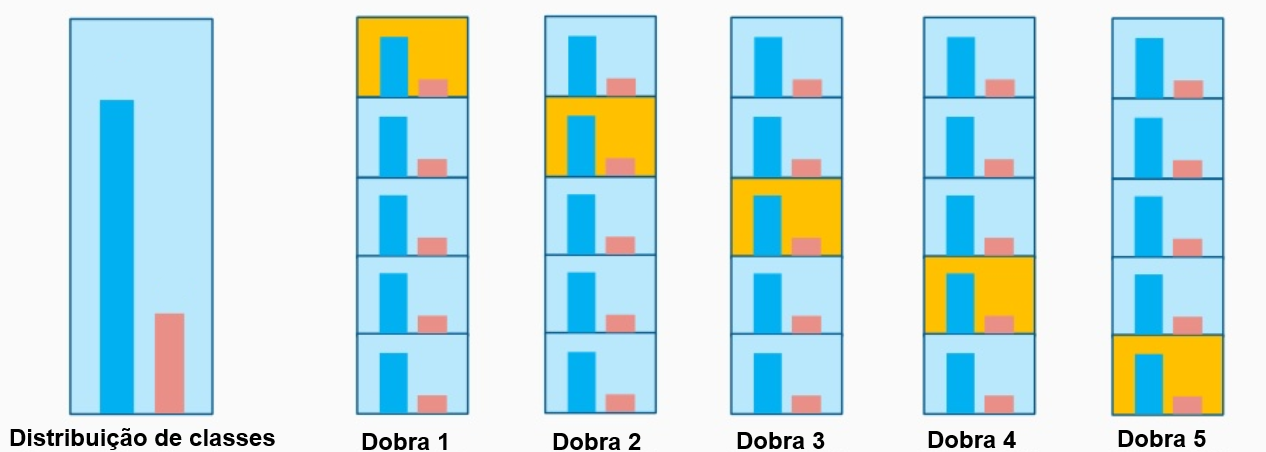
\includegraphics[width=0.9\linewidth]{Figures/kfold.png}
    \caption{Esquema de particionamento estratificado em nível de paciente (variante \textit{fold-wise} de 5 dobras).}
    \label{kfold}
\end{figure}

\subsection{Treinamento do modelo de classificação}

O conjunto de dados real foi submetido a uma etapa de \textit{downsampling} das amostras benignas, a fim de reduzir o desbalanceamento entre as classes. Especificamente, o número de imagens benignas de DEV foi reduzido para igualar o de malignas, resultando em 194 amostras por classe (388 imagens no total), mantendo todas as instâncias malignas disponíveis. Essa redução foi realizada de forma aleatória, com \textit{seed} fixa e de maneira consciente ao paciente, garantindo reprodutibilidade e evitando a divisão de uma mesma paciente no corte de balanceamento. Em seguida, as imagens sintéticas geradas pelo modelo \textit{StyleGAN2-ADA} foram adicionadas apenas ao conjunto de treinamento de DEV, preservando tanto a validação interna quanto o conjunto de teste bloqueado compostos exclusivamente por imagens reais.

Durante o treinamento, a rede \textit{EfficientNet-B0} foi inicializada com pesos pré-treinados no \textit{ImageNet}, e apenas a camada de classificação foi substituída por um neurônio de saída com ativação sigmoide, apropriada para o problema binário (benigno/maligno). No modelo reportado, toda a rede foi ajustada por \textit{fine-tuning}, com a base convolucional destravada, de modo a adaptar as representações ao domínio das mamografias. O treinamento foi conduzido com o otimizador \textit{Adam}, taxa de aprendizado de $1 \times 10^{-4}$ e função de perda \textit{Binary Cross-Entropy with Logits (BCEWithLogitsLoss)}. Como ablação, avaliou-se também uma configuração com a base convolucional congelada, treinando apenas a camada de classificação, que apresentou desempenho próximo ao acaso (AUC $\approx 0{,}545$), confirmando a necessidade de um classificador funcional para mensurar o efeito das imagens sintéticas.

Cada época (\textit{epoch}), que corresponde a uma passagem completa por todo o conjunto de treinamento, processou lotes de 32 imagens com aumento de dados aplicado em tempo real. As transformações incluíram rotações aleatórias de até $5^{\circ}$ e inversão horizontal, contribuindo para maior robustez do modelo frente à variação posicional das estruturas mamárias. O carregamento dos dados foi realizado com duas \textit{threads} paralelas e memória pinada (\textit{pinned memory}), técnica que fixa os dados na RAM para otimizar a transferência entre CPU e GPU, reduzindo a latência no carregamento dos lotes durante o treinamento.

O treinamento foi executado por até 30 épocas, com monitoramento contínuo das métricas de acurácia, F1-\textit{score} e AUC. Ao final de cada época, o modelo era avaliado na validação interna de DEV, sendo armazenados os melhores pesos e aplicada parada antecipada com base no desempenho obtido; a avaliação definitiva de cada modelo foi realizada uma única vez sobre o conjunto de teste bloqueado. No protocolo principal, esse procedimento foi repetido por 10 sementes independentes para cada proporção, resultando em uma distribuição de métricas de teste que fundamenta a análise estatística. Toda a execução foi realizada em uma GPU, utilizando precisão mista (\textit{mixed precision}) para reduzir o consumo de memória e acelerar o processamento.
 
\subsection{Métricas de classificação}

Para avaliar o desempenho do modelo \textit{EfficientNet-B0} no problema de detecção de lesões mamográficas, foram empregadas métricas consolidadas na literatura de aprendizado de máquina para tarefas de classificação binária: acurácia, F1-score e área sob a curva ROC (AUC).

A acurácia mede a proporção total de predições corretas em relação ao número total de amostras avaliadas, e é uma métrica global definida pela equação \eqref{eq31}:

\begin{equation}
\text{Acurácia} = \frac{TP + TN}{TP + TN + FP + FN},
\label{eq31}
\end{equation}

\noindent onde $TP$ (verdadeiros positivos) representa o número de lesões malignas corretamente classificadas, $TN$ (verdadeiros negativos) o número de amostras benignas corretamente identificadas, $FP$ (falsos positivos) o número de amostras benignas classificadas incorretamente como malignas e $FN$ (falsos negativos) o número de amostras malignas preditas como benignas.

O F1-score, por sua vez, é a média harmônica entre a precisão (\textit{precision}) e a revocação (\textit{recall}), sendo especialmente útil em cenários de classes desbalanceadas, como é comum em bases médicas. Suas definições são dadas pela equação \eqref{eq32}:

\begin{equation}
\text{Precisão} = \frac{TP}{TP + FP}, \quad
\text{Revocação} = \frac{TP}{TP + FN},
\label{eq32}
\end{equation}

\noindent e o F1-score é calculado pela equação \eqref{eq33}:

\begin{equation}
\text{F1-score} = 2 \times \frac{\text{Precisão} \times \text{Revocação}}{\text{Precisão} + \text{Revocação}}.
\label{eq33}
\end{equation}

Essa métrica, equação \eqref{eq33}, penaliza fortemente classificações incorretas em qualquer uma das classes, equilibrando a capacidade do modelo de detectar casos positivos (revocação) e evitar alarmes falsos (precisão).

Já a área sob a curva ROC (AUC — \textit{Area Under the Curve}) quantifica a capacidade discriminatória do modelo ao variar o limiar de decisão. A curva ROC (\textit{Receiver Operating Characteristic}) é construída a partir da relação entre a taxa de verdadeiros positivos (TPR) e a taxa de falsos positivos (FPR), definidas pela equação \eqref{eq34}:

\begin{equation}
\text{TPR} = \frac{TP}{TP + FN}, \quad
\text{FPR} = \frac{FP}{FP + TN}.
\label{eq34}
\end{equation}

A métrica AUC é então calculada como a integral da curva ROC, conforme mostrado na equação \eqref{eq35}:

\begin{equation}
\text{AUC} = \int_{0}^{1} \text{TPR}(\text{FPR}) \, d(\text{FPR}).
\label{eq35}
\end{equation}

Essa integral representa a área sob a curva ROC, assumindo valores entre 0 e 1. Um modelo com $\text{AUC} = 0.5$ equivale a uma classificação aleatória, enquanto valores próximos de 1 indicam excelente separabilidade entre as classes.

As métricas foram calculadas sobre o conjunto de teste bloqueado para cada uma das sementes e posteriormente agregadas por média e desvio padrão, fornecendo uma estimativa da performance do modelo por proporção.

\subsection{Análise estatística}
\label{sec:analise_estatistica}

Como o classificador é treinado sob múltiplas sementes, cada proporção sintético:real gera uma distribuição de métricas no conjunto de teste, o que permite uma análise estatística das diferenças de desempenho. Para cada proporção, reporta-se a média e o desvio padrão acompanhados de um intervalo de confiança de 95\% obtido por \textit{bootstrap}. A comparação de cada proporção com a linha de base composta apenas por dados reais é feita com o teste de Wilcoxon pareado (\textit{signed-rank}), utilizando as mesmas sementes, com correção de Holm para múltiplas comparações. O tamanho de efeito é quantificado pelo delta de Cliff, e as diferenças de AUC são avaliadas pelo teste de DeLong \cite{delong1988} sobre as predições agregadas do conjunto de teste. Um resultado só é considerado uma melhoria efetiva quando é, simultaneamente, consistente entre as sementes e estatisticamente significativo após a correção.


\chapter{Resultados}

Este capítulo apresenta e discute os resultados obtidos a partir dos experimentos realizados com os modelos de geração e classificação de imagens de mamografia. Inicialmente, são descritos os resultados referentes à geração de imagens sintéticas utilizando o modelo StyleGAN2-ADA, com análise baseada na métrica perceptual LPIPS para avaliar a qualidade e a similaridade das amostras geradas em relação às imagens reais.

Em seguida, são apresentados os resultados da classificação de mamografias empregando o modelo EfficientNet-B0, incluindo a avaliação do impacto da incorporação de imagens sintéticas no desempenho do classificador. As métricas de acurácia, F1-score e AUC são analisadas de forma comparativa, buscando identificar a proporção ideal entre dados reais e sintéticos que maximize a performance do modelo. Por fim, são discutidas as implicações dos resultados obtidos, bem como as limitações e observações relevantes quanto à viabilidade computacional dos experimentos realizados.

\section{Geração de imagens de mamografia}

O gerador StyleGAN2-ADA foi treinado com um conjunto relativamente reduzido de 439 imagens reais pertencentes exclusivamente à partição de desenvolvimento (DEV), com predominância de exemplos benignos sobre malignos. Essa limitação de amostras representa um desafio relevante, principalmente pela disparidade entre as classes, que pode afetar a capacidade do modelo de capturar adequadamente as variações presentes nas imagens malignas.

A análise da distribuição dos valores LPIPS, Figura \ref{resultados_lpips}, na geração de 1000 imagens para classe benigna e 1000 para maligna, mostra que a maioria das imagens geradas apresenta alta similaridade perceptual em relação às imagens reais. A distribuição geral apresenta média de 0.247 e mediana de 0.249, com concentração em torno de 0.25, indicando que o gerador manteve um padrão de qualidade estável ao longo das amostras. A proximidade entre média e mediana sugere uma distribuição simétrica, sem a presença de valores extremos significativos.

Ao observar a distribuição por classe, Figura \ref{distr_class_lpips}, nota-se que as imagens malignas tendem a apresentar valores de LPIPS ligeiramente mais altos em comparação às benignas. Esse comportamento pode estar diretamente relacionado à menor quantidade de exemplos malignos disponíveis no treinamento, o que limita a capacidade do modelo em generalizar os padrões dessa classe. Como consequência, o gerador produz imagens malignas com maior variabilidade estrutural e, portanto, diferenças perceptuais um pouco mais pronunciadas em relação às imagens reais. Essa tendência é corroborada pela curva de densidade de probabilidade, onde as imagens malignas exibem distribuição mais ampla, indicando maior dispersão dos valores LPIPS.

\begin{figure}[H]
    \centering
    % Subfigura (a)
    \begin{subfigure}[b]{0.45\textwidth}
        \centering
        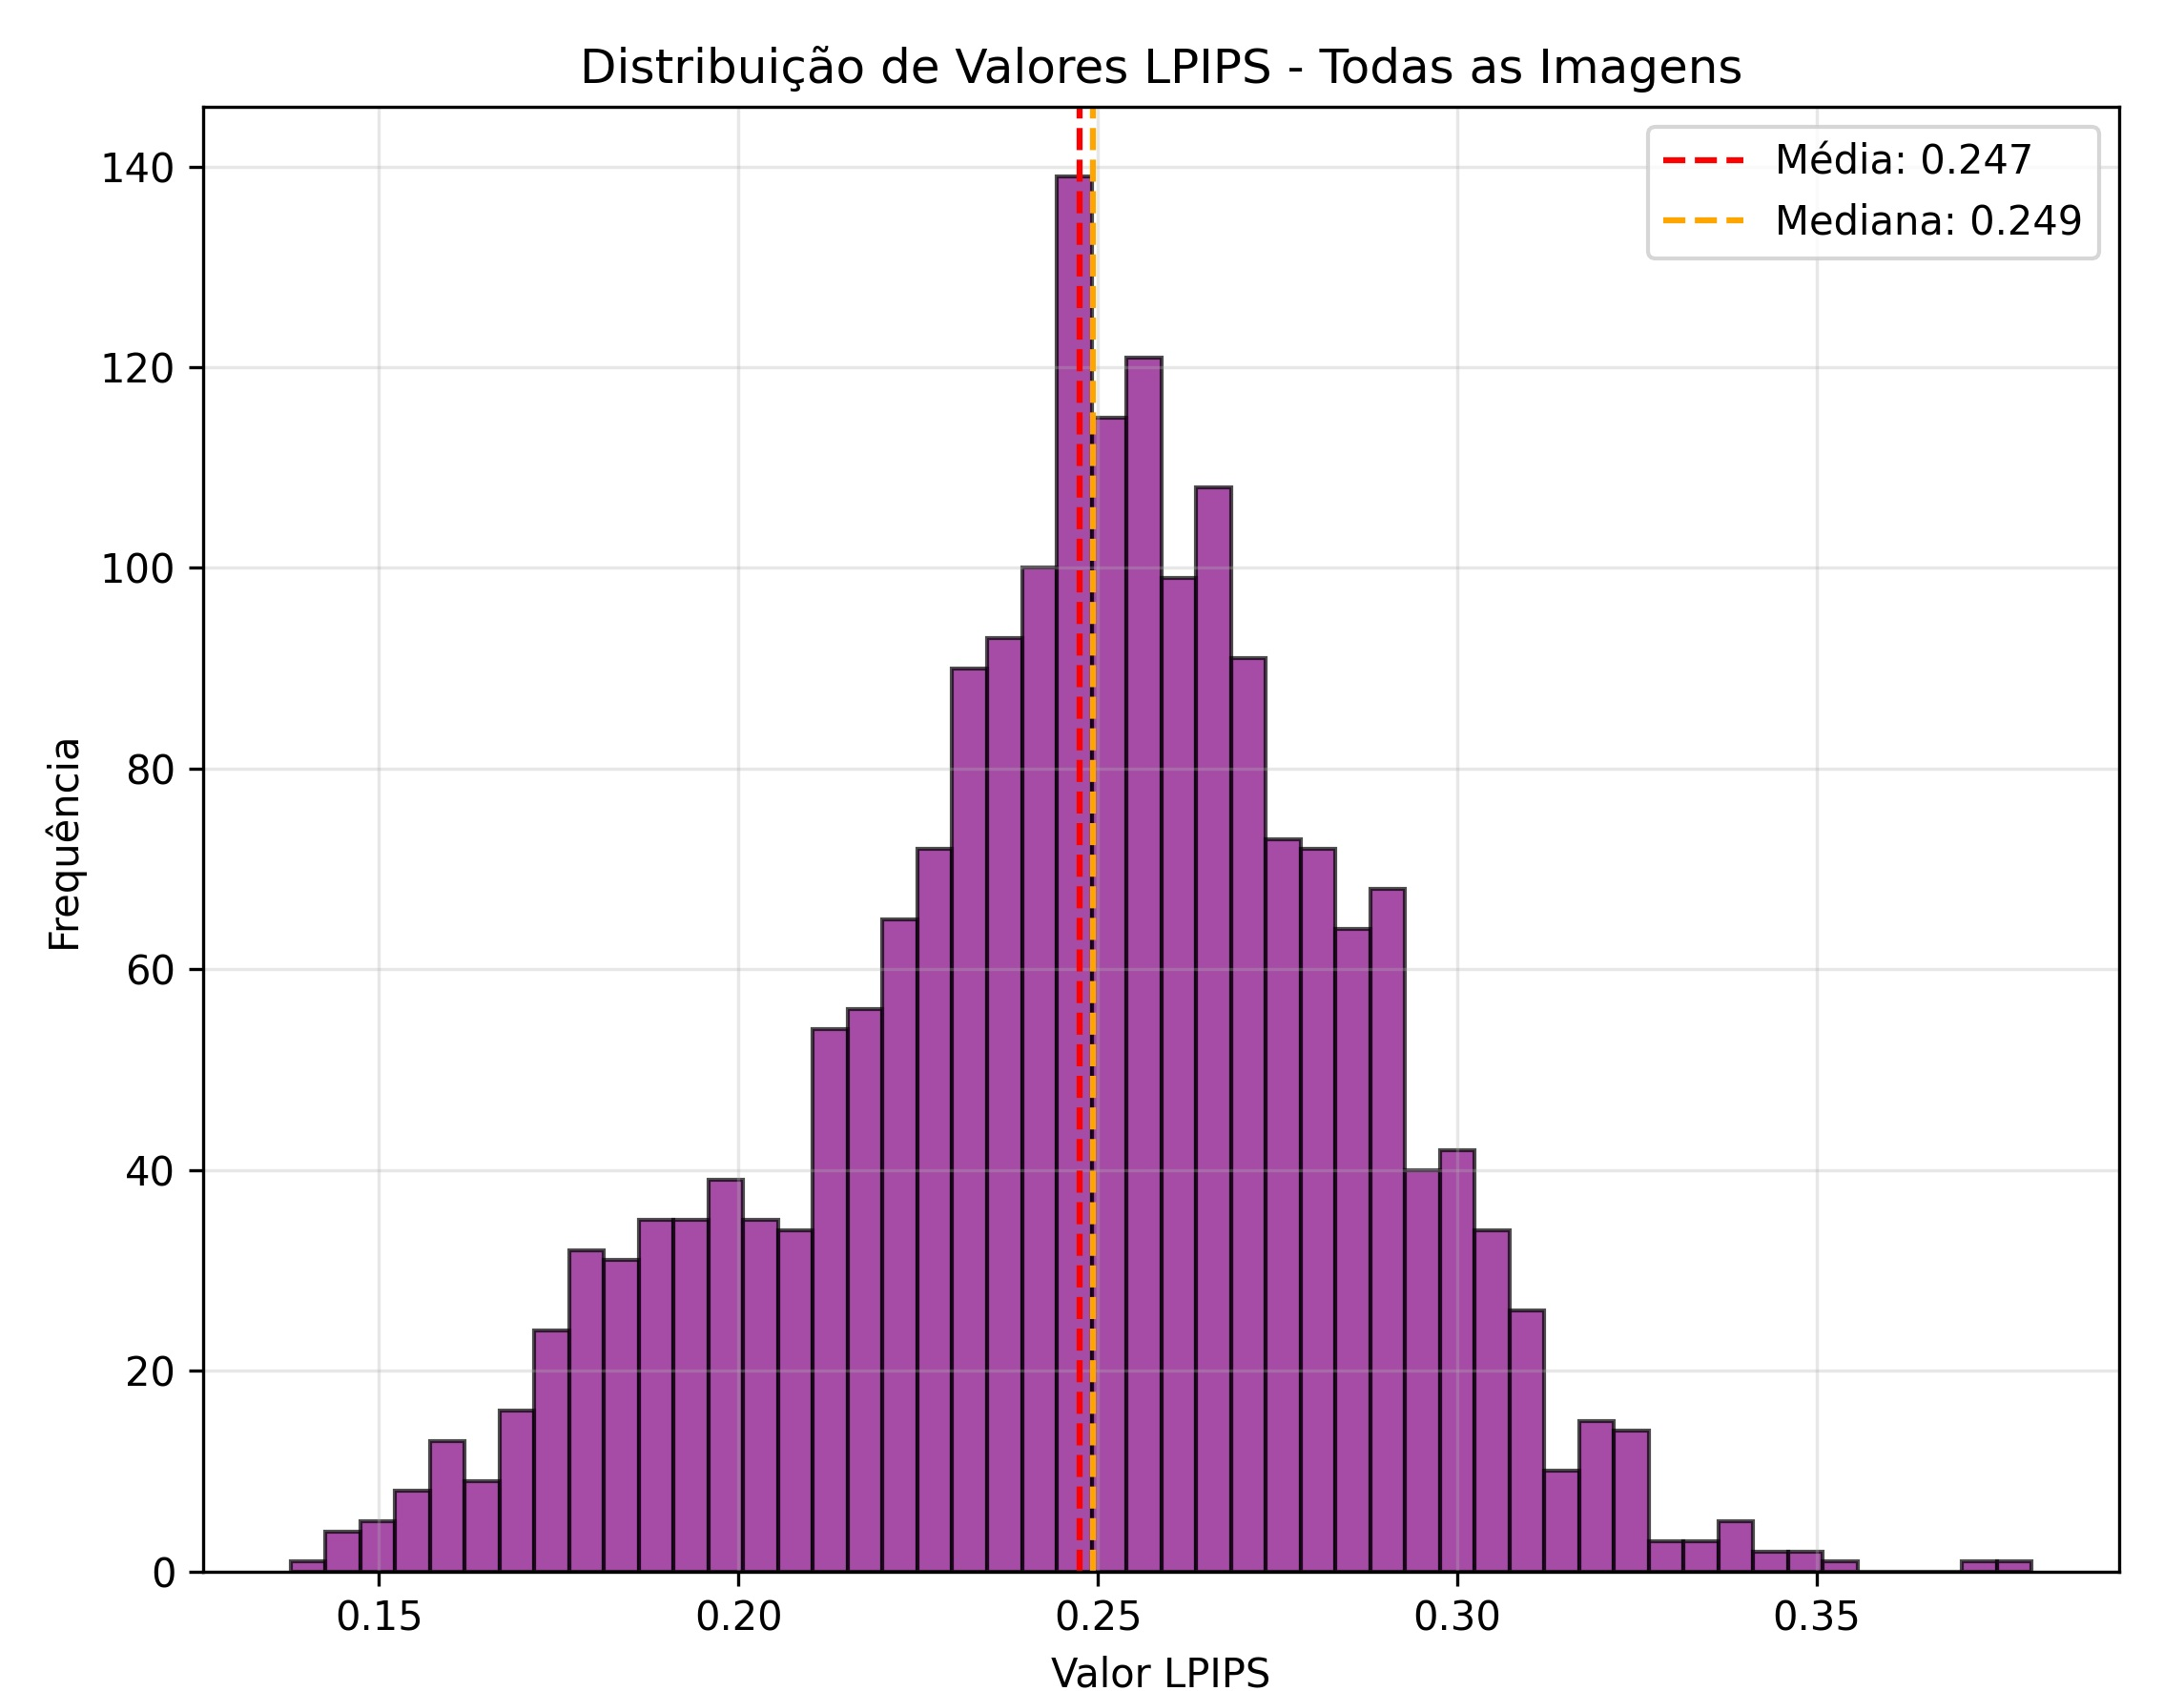
\includegraphics[width=\textwidth]{Figures/distr_lpips.jpg}
        \caption{Distribuição LPIPS para todas as imagens}
        \label{distr_lpips}
    \end{subfigure}
    \hfill
    % Subfigura (b)
    \begin{subfigure}[b]{0.45\textwidth}
        \centering
        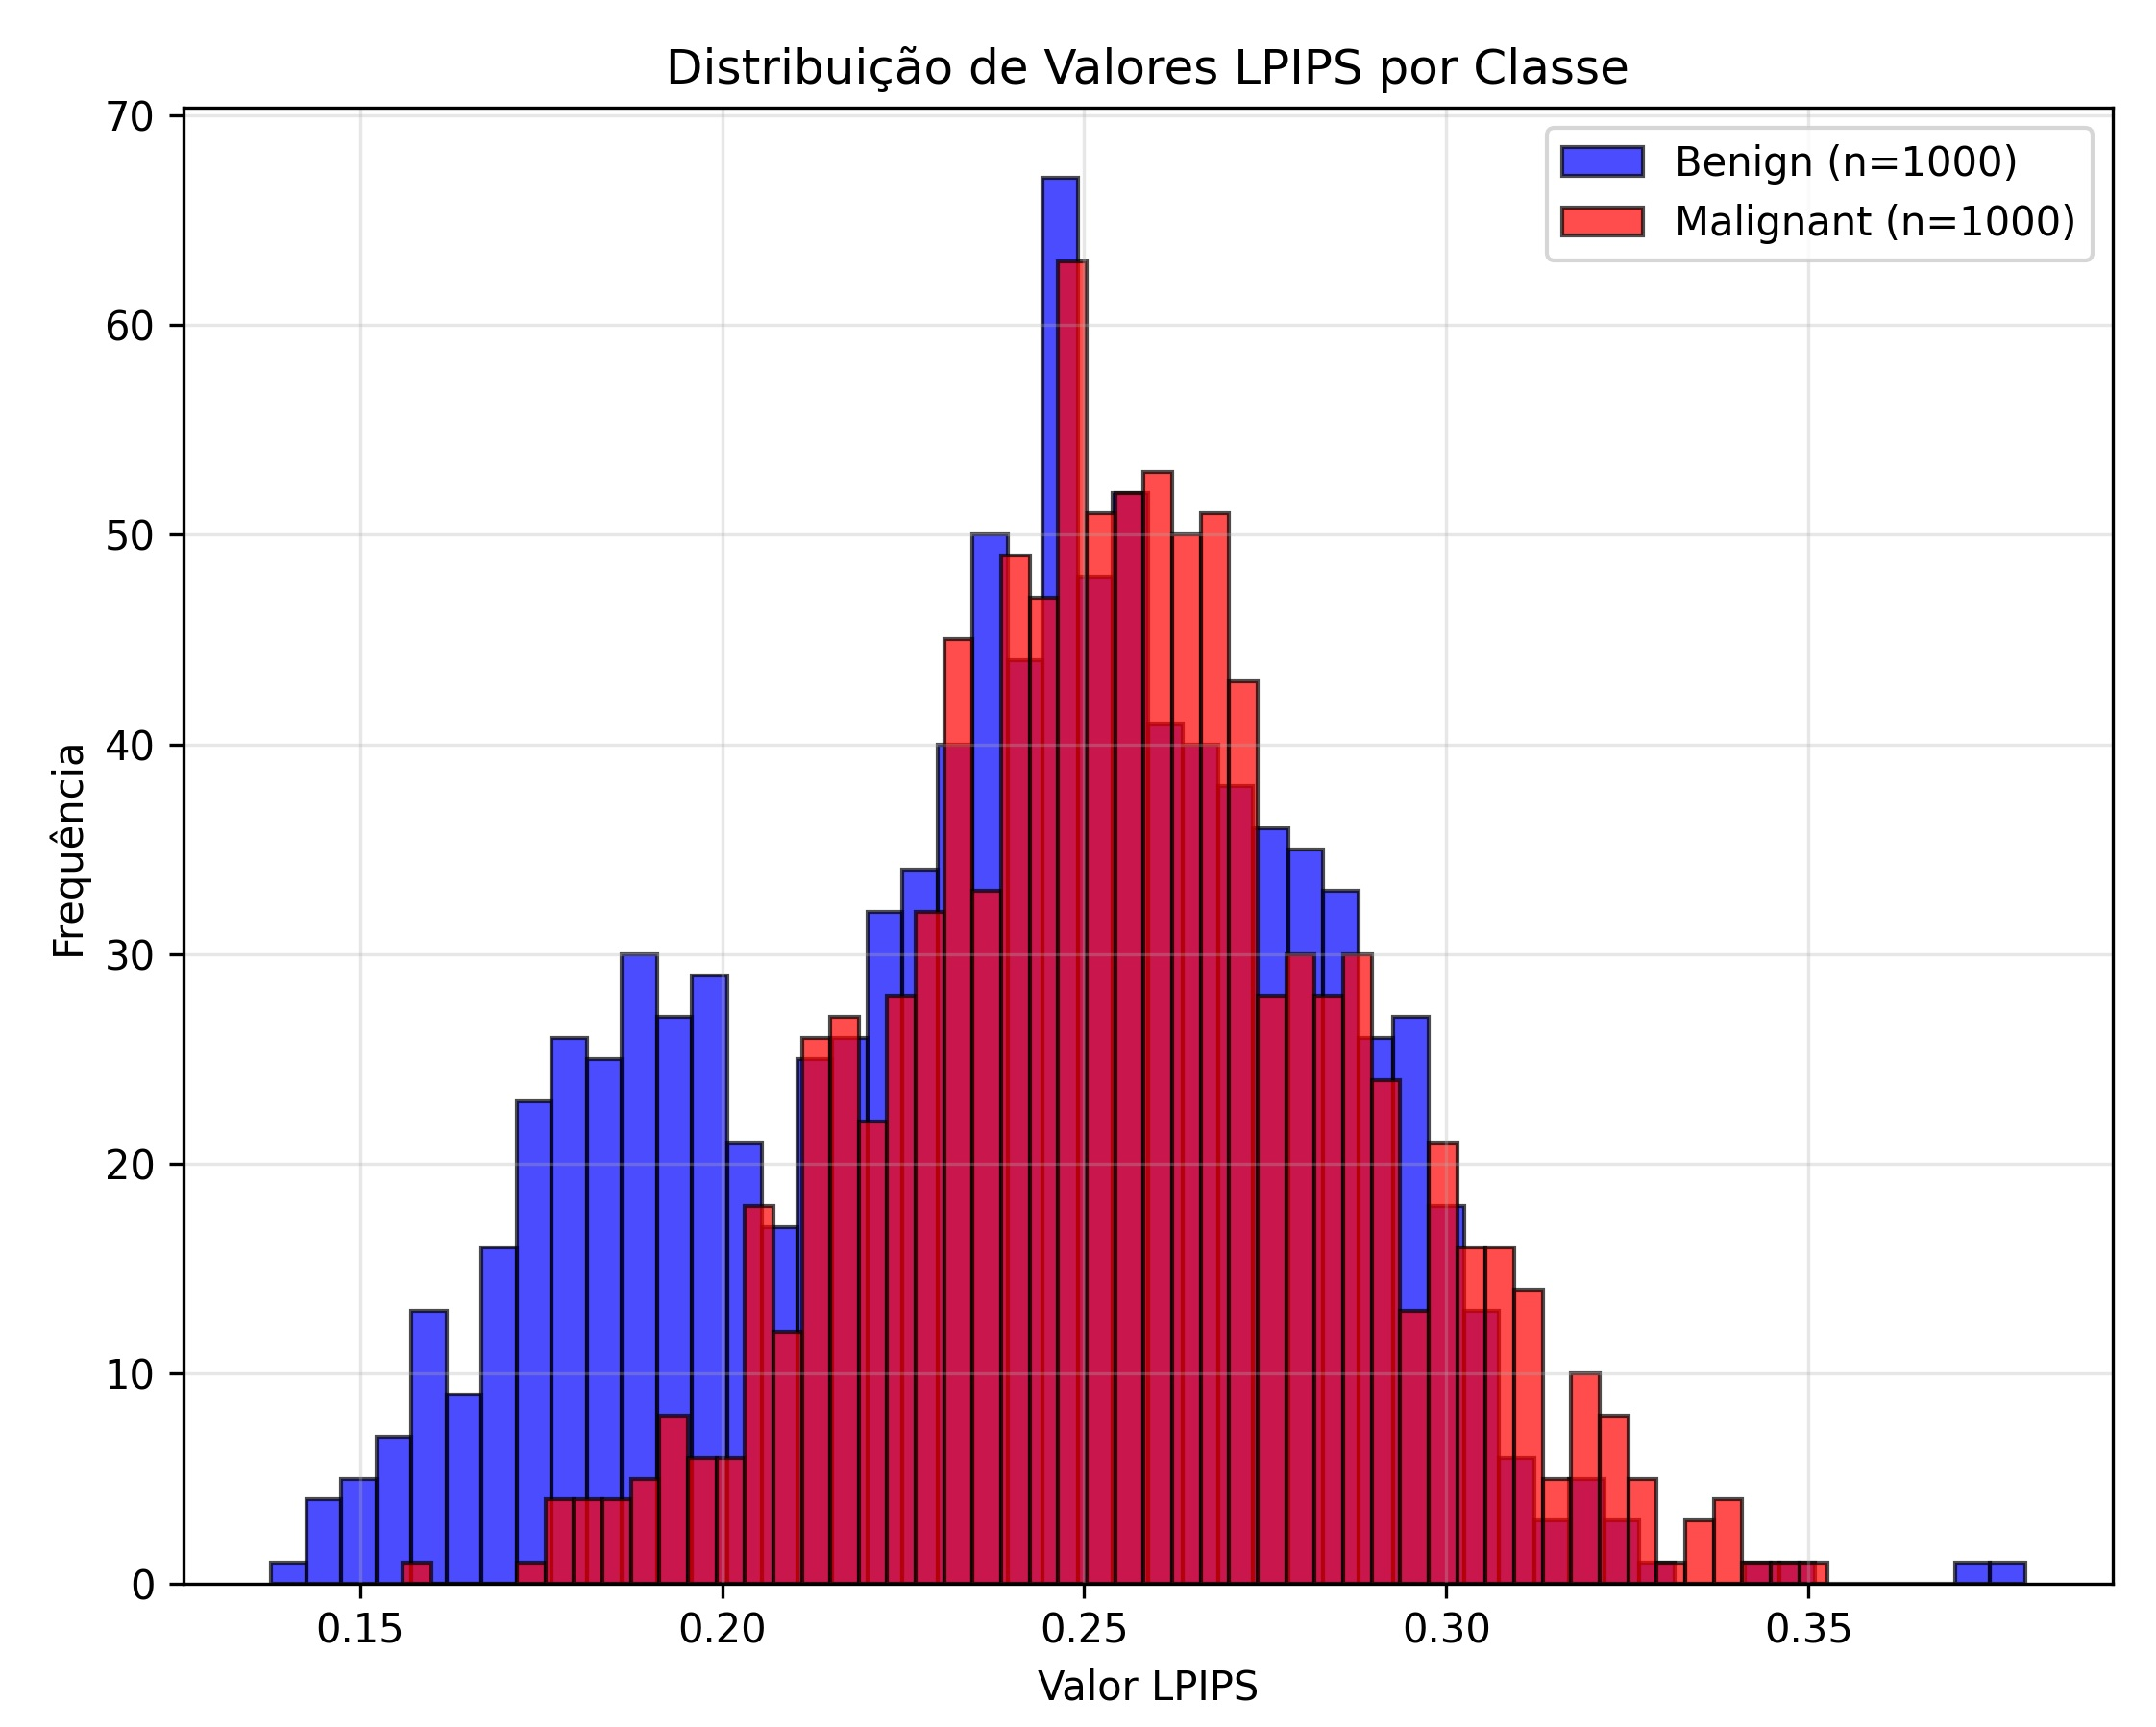
\includegraphics[width=\textwidth]{Figures/distr_class_lpips.jpg}
        \caption{Distribuição LPIPS para cada classe de imagem}
        \label{distr_class_lpips}
    \end{subfigure}
    % Subfigura (c)
    \begin{subfigure}[b]{0.45\textwidth}
        \centering
        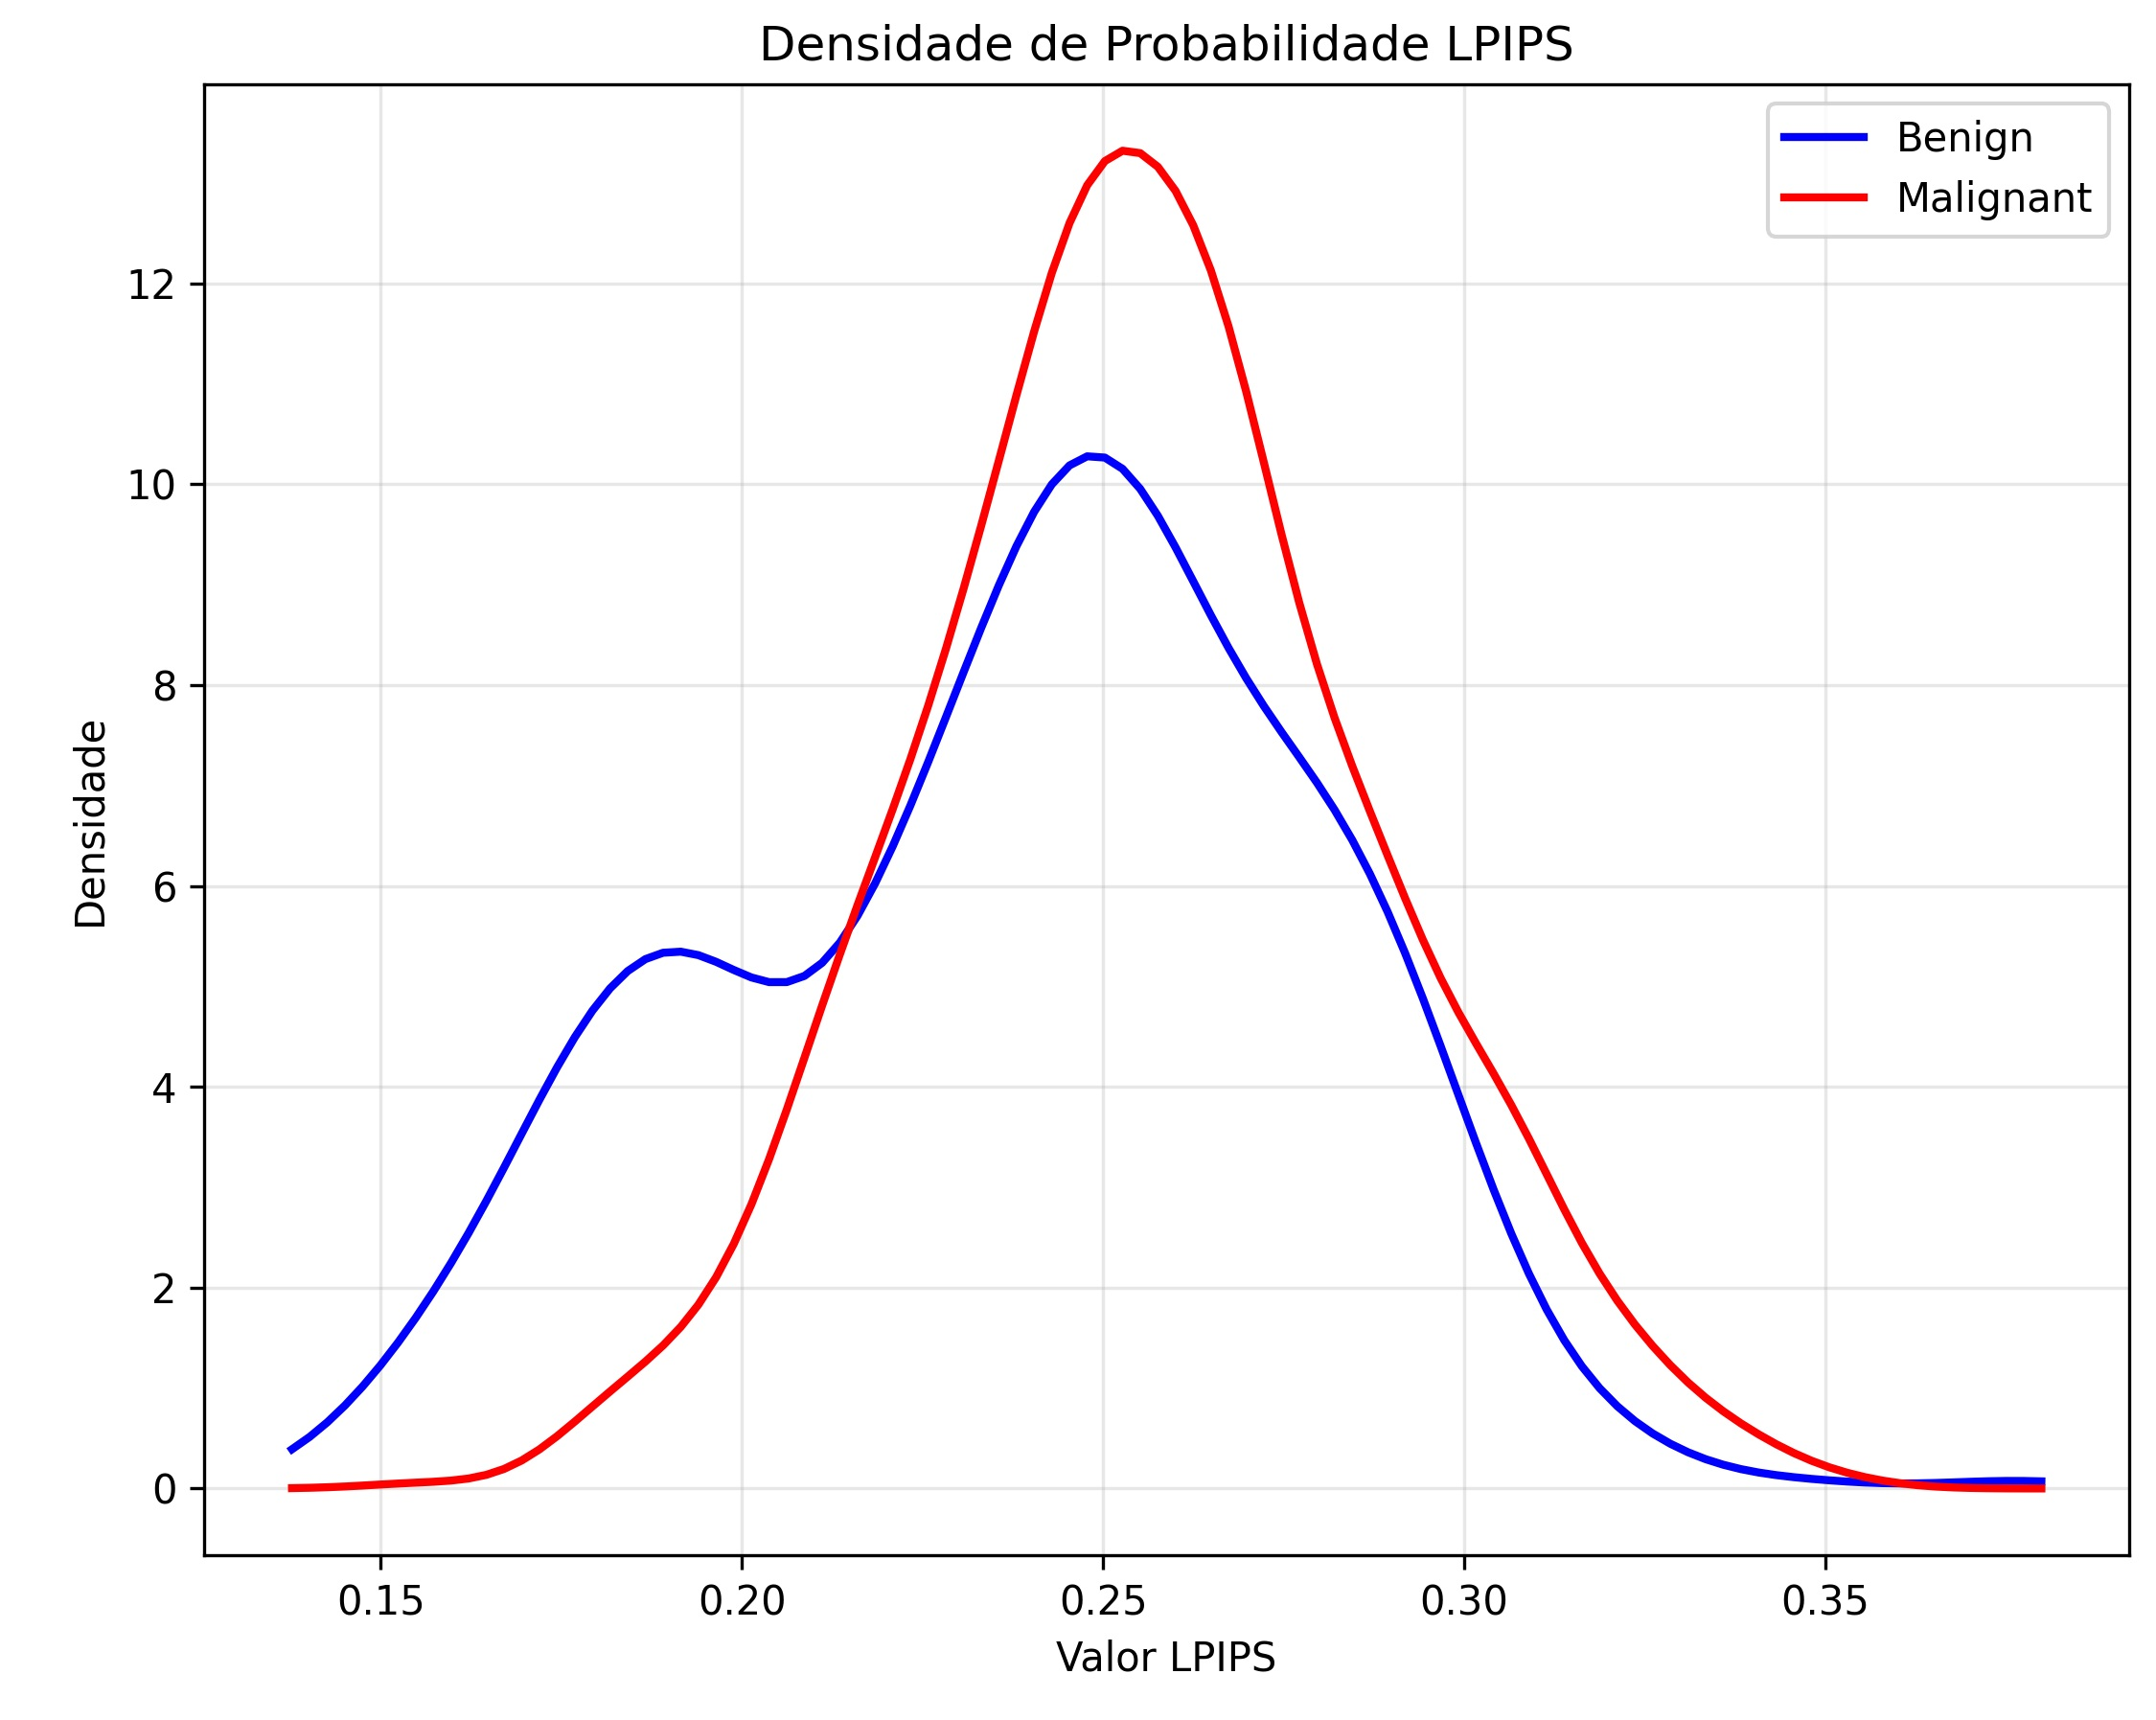
\includegraphics[width=\textwidth]{Figures/dens_lpips.jpg}
        \caption{Densidade LPIPS}
        \label{dens_lpips}
    \end{subfigure}
    \hfill
    % Subfigura (d)
    \begin{subfigure}[b]{0.45\textwidth}
        \centering
        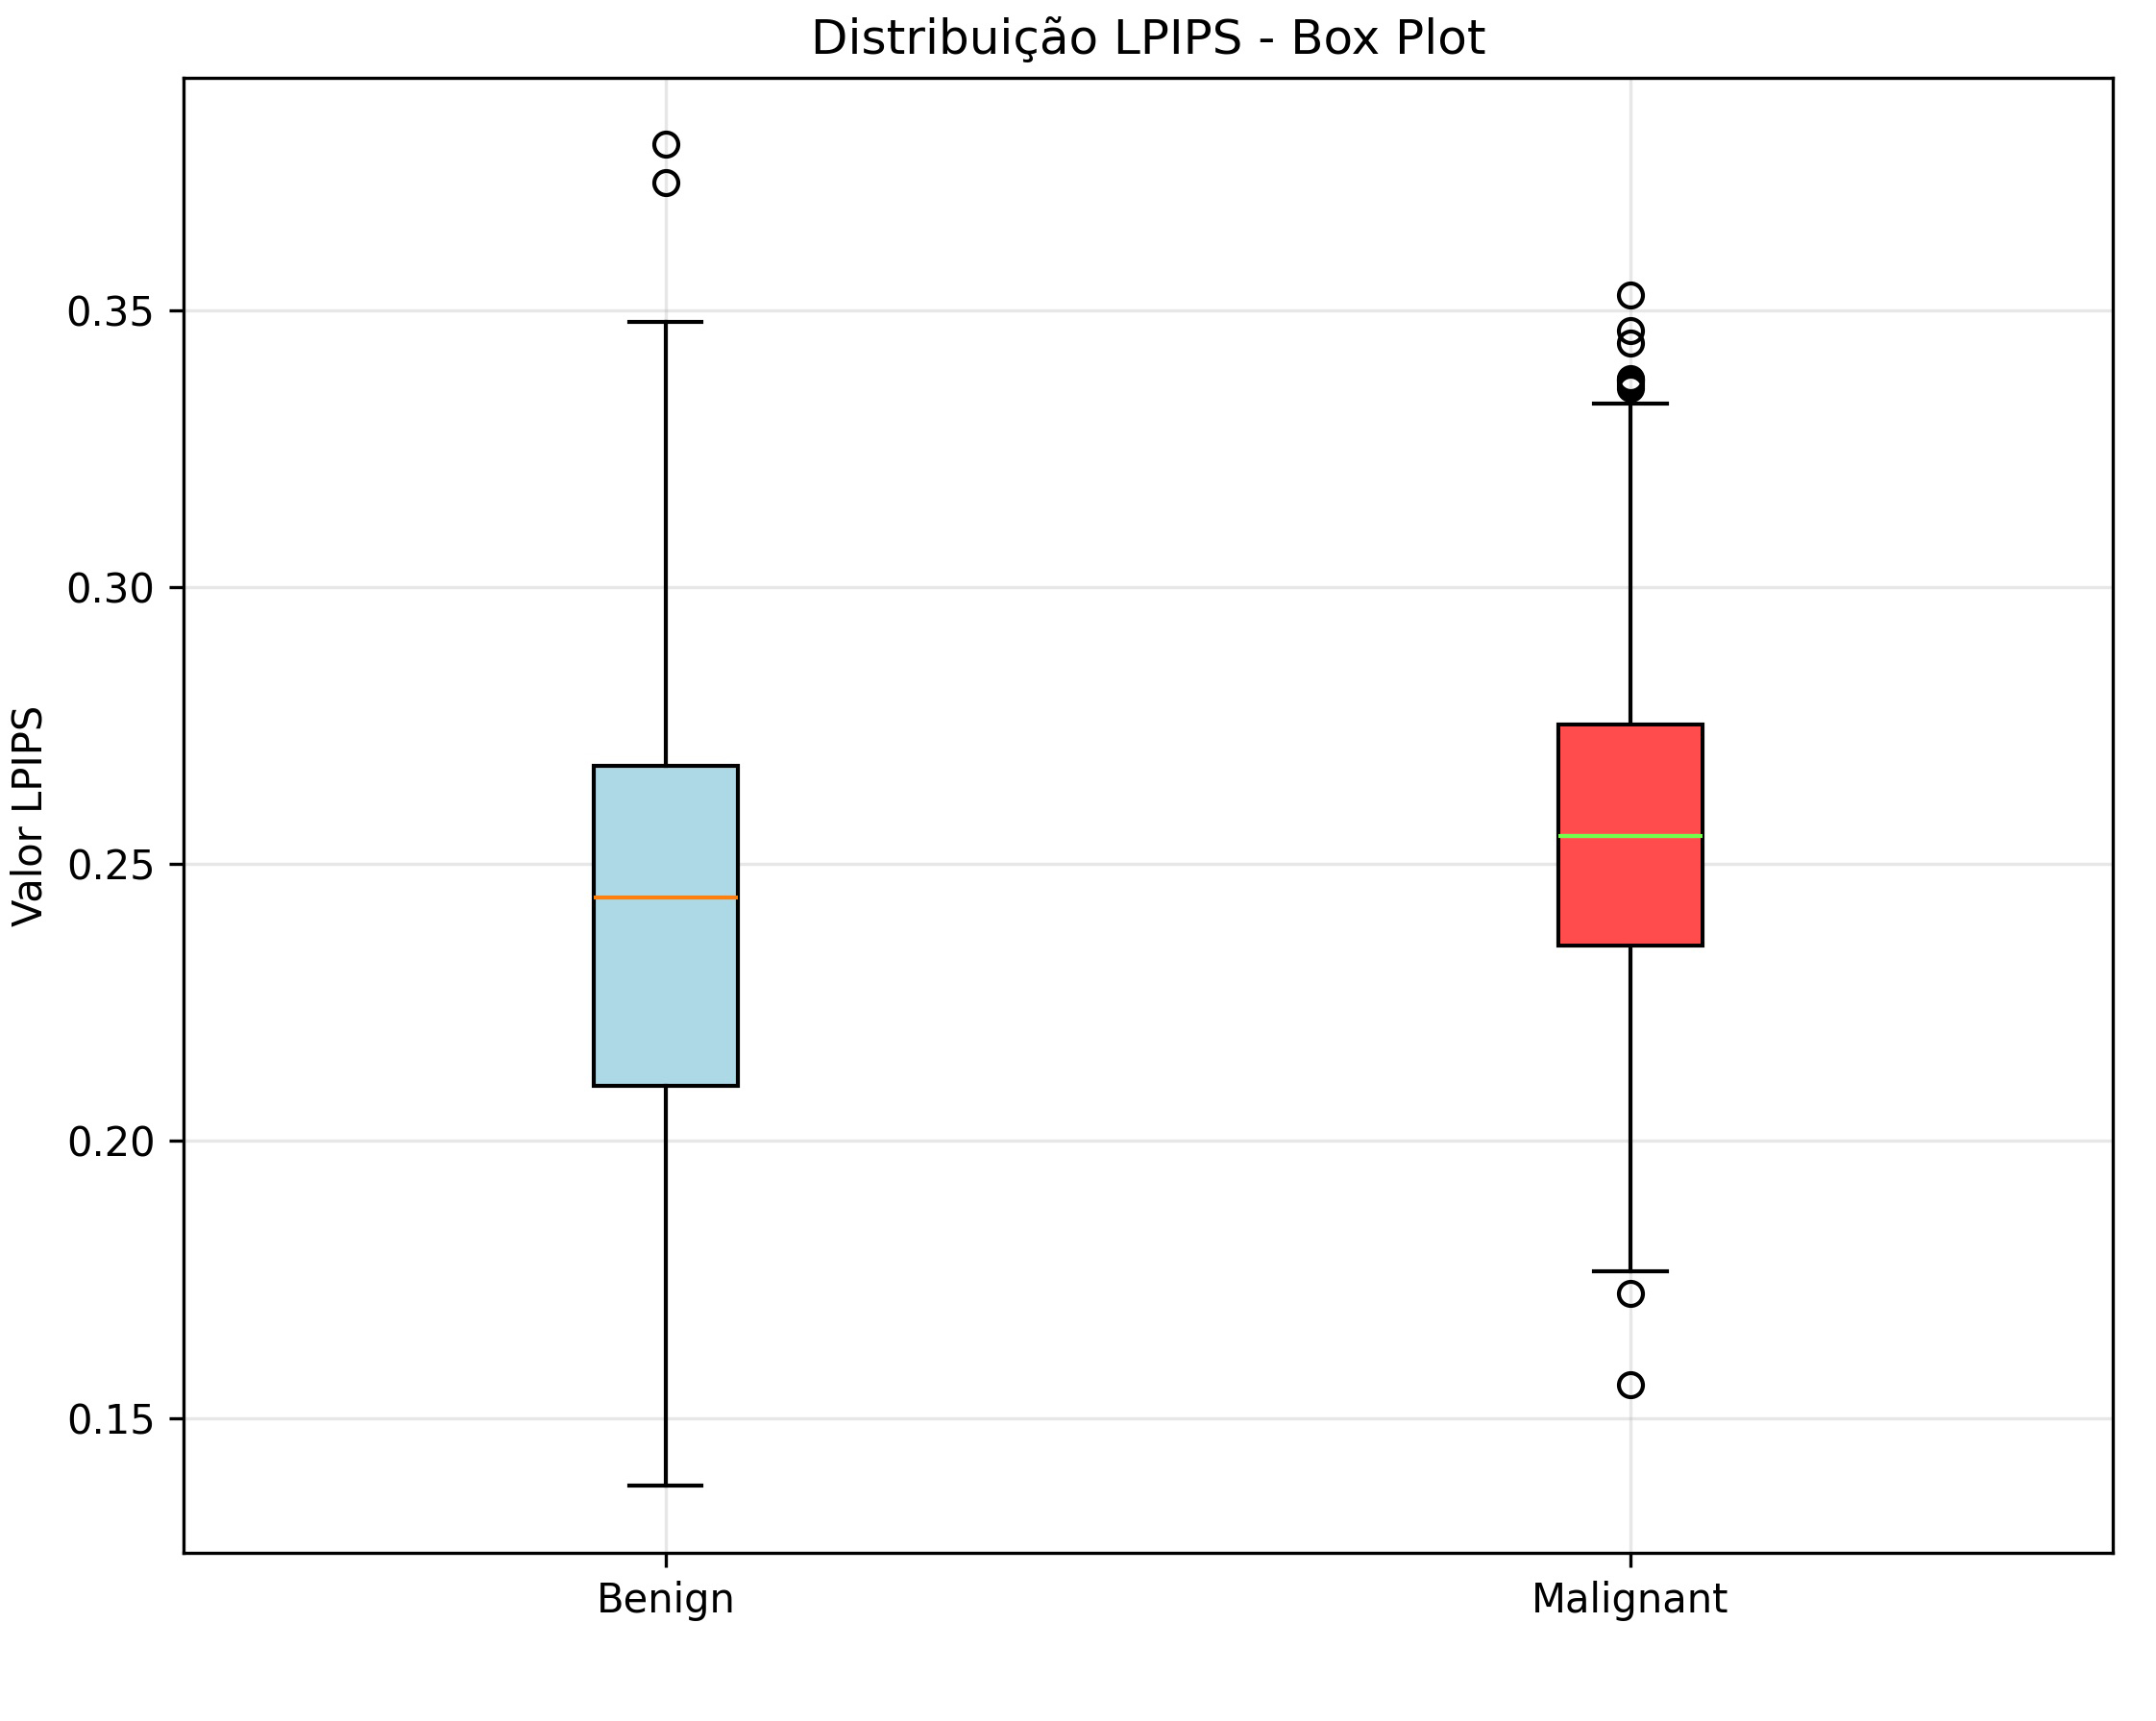
\includegraphics[width=\textwidth]{Figures/box_lpips.jpg}
        \caption{Box plot LPIPS}
        \label{box_lpips}
    \end{subfigure}

    \caption{Gráficos dos valores do LPIPS na geração de 1000 imagens para cada classe usando StyleGAN2-ADA. Em laranja estão representadas as classes malignas e em azul as benignas.}
    \label{resultados_lpips}
\end{figure}

Mesmo com essa diferença, a sobreposição significativa entre as distribuições das duas classes e a proximidade das medianas no box plot, Figura \ref{box_lpips}, demonstram que o modelo manteve uma qualidade perceptual consistente entre as categorias. A presença de poucos outliers e a amplitude interquartílica semelhante reforçam a estabilidade do processo de geração, apesar do número reduzido de imagens reais utilizadas para o treinamento.

Como o LPIPS, isoladamente, não é suficiente para detectar baixa diversidade ou memorização das amostras, a avaliação da geração foi complementada pelas métricas \textit{Fréchet Inception Distance} (FID) \cite{heusel2017fid} e \textit{Kernel Inception Distance} (KID) \cite{binkowski2018kid}, calculadas por classe entre as imagens reais de DEV e as imagens sintéticas. Diferentemente do LPIPS, que compara pares individuais de imagens, o FID e o KID comparam as distribuições de características extraídas por uma rede pré-treinada, oferecendo uma medida agregada de fidelidade e diversidade que complementa a análise perceptual \cite{zhang2018lpips}.

A análise quantitativa da geração confirmou a adequação do ponto de operação adotado. A varredura de limiares mostrou que o valor $\tau = 0{,}2$, empregado no trabalho original, tornou-se inviável sob o protocolo livre de vazamento, uma vez que resultou em retenção nula de amostras da classe maligna (0\%); adotou-se, portanto, $\tau = 0{,}25$, que produziu aceitação de 26\% para a classe benigna e 8\% para a maligna, enquanto $\tau = 0{,}3$ elevava a aceitação para cerca de 64\% em ambas as classes, à custa de menor fidelidade. A verificação de memorização não sinalizou nenhuma amostra (0\%, $n_{\text{sinalizadas}} = 0$): o menor valor de LPIPS entre as imagens retidas e seus vizinhos reais mais próximos foi de 0,226 para a classe benigna e 0,235 para a maligna, com mínimo absoluto de 0,175, valores bem acima do limiar de memorização de 0,05. Quanto à fidelidade e à diversidade agregadas, obteve-se FID de 162,9 (benigno) e 166,2 (maligno) e KID de $0{,}138 \pm 0{,}007$ (benigno) e $0{,}151 \pm 0{,}011$ (maligno), valores compatíveis com o tamanho reduzido do conjunto de treinamento (439 imagens reais de DEV) e com a resolução de $128 \times 128$ pixels.

\section{Classificação de mamografias}

Os resultados da avaliação perceptual sugerem que o modelo generativo reproduziu de forma razoável a distribuição visual das mamografias reais, com fidelidade perceptual coerente com o tamanho reduzido do conjunto. Essa coerência visual indica que as imagens produzidas preservam características estruturais relevantes das mamografias reais, o que motiva investigar sua utilização como complemento no treinamento de modelos de classificação. Assim, procedeu-se à etapa de avaliação quantitativa, na qual se investigou o impacto da inclusão dessas imagens sintéticas no desempenho do classificador \textit{EfficientNet-B0}.

Após a seleção das imagens sintéticas por meio da varredura de limiares LPIPS, o impacto da sua utilização no treinamento do modelo \textit{EfficientNet-B0} foi avaliado sob o protocolo de \textit{hold-out} em nível de paciente descrito na Seção~\ref{sec:protocolo}. O gerador e o filtro perceptual tiveram acesso apenas ao conjunto DEV; o classificador foi treinado sobre a combinação de imagens reais e sintéticas de DEV, com seleção de modelo em uma validação interna, e avaliado sobre o conjunto TEST bloqueado. O procedimento foi repetido por 10 sementes independentes para cada proporção, assegurando que a mensuração de desempenho não fosse contaminada por imagens vistas nas etapas de geração ou de filtragem.

Sob o protocolo corrigido, livre de vazamento, os resultados quantitativos definitivos foram obtidos após a reexecução completa da \textit{pipeline}, com 10 sementes independentes e avaliação sobre o conjunto de teste bloqueado ($n = 98$). Os números da versão anterior, provenientes do arranjo com vazamento de dados, não são reaproveitados nem apresentados como válidos. A Tabela~\ref{tab:efficientnet_results} apresenta as métricas de teste (média e intervalo de confiança de 95\%) para cada proporção. O classificador reportado corresponde ao modelo ajustado por \textit{fine-tuning}, com a base convolucional da \textit{EfficientNet-B0} destravada; a variante com a base congelada, treinando apenas a cabeça linear, permanece próxima ao acaso (AUC $\approx 0{,}545$) e é reportada apenas como ablação, evidenciando que um classificador funcional é necessário para mensurar o efeito das imagens sintéticas.

\begin{table}[H]
\centering
\caption{Resultados no conjunto de teste bloqueado (EfficientNet-B0), sob o protocolo livre de vazamento (média e intervalo de confiança de 95\% por \textit{bootstrap}, 10 sementes, $n = 98$). As proporções 2:1 e 3:1, destacadas em negrito, apresentaram os melhores resultados.}
\label{tab:efficientnet_results}
\renewcommand{\arraystretch}{1.2}
\begin{tabularx}{0.95\textwidth}{l *{3}{>{\centering\arraybackslash}X}}
\toprule
\textbf{Proporção} & \textbf{Acurácia (IC 95\%)} & \textbf{F1-Score (IC 95\%)} & \textbf{AUC (IC 95\%)} \\ \midrule
Apenas reais (0:1) & 0,566 [0,544; 0,588] & 0,527 [0,493; 0,563] & 0,611 [0,583; 0,645] \\
1:1 & 0,611 [0,593; 0,630] & 0,574 [0,533; 0,614] & 0,659 [0,649; 0,669] \\
\textbf{2:1} & \textbf{0,619 [0,598; 0,642]} & \textbf{0,574 [0,522; 0,619]} & \textbf{0,682 [0,666; 0,699]} \\
\textbf{3:1} & \textbf{0,634 [0,611; 0,653]} & \textbf{0,598 [0,560; 0,634]} & \textbf{0,683 [0,665; 0,701]} \\
4:1 & 0,614 [0,599; 0,633] & 0,568 [0,526; 0,613] & 0,676 [0,655; 0,696] \\
\bottomrule
\end{tabularx}
\end{table}

\begin{quote}
\footnotesize \textit{Observação:} os valores da Tabela~\ref{tab:efficientnet_results} provêm da reexecução da \textit{pipeline} sob o protocolo livre de vazamento (\textit{hold-out} em nível de paciente, 10 sementes), substituindo integralmente os números da versão anterior, obtidos sob arranjo com vazamento de dados.
\end{quote}

A análise comparativa entre proporções, conduzida sobre as métricas regeneradas com os testes formais descritos na Seção~\ref{sec:analise_estatistica}, revela um padrão consistente. Em relação à linha de base composta apenas por dados reais, o ganho de AUC foi estatisticamente significativo em todas as proporções pelo teste de Wilcoxon pareado com correção de Holm ($p_{\text{aj}} = 0{,}047$), acompanhado de tamanhos de efeito grandes (delta de Cliff entre 0,72 e 0,80). A acurácia também melhorou de forma significativa em todas as proporções ($p_{\text{aj}}$ entre 0,008 e 0,025). Já o F1-\textit{score} não atingiu significância estatística em nenhuma proporção (menor $p_{\text{aj}} \approx 0{,}055$, observado em 3:1). O teste de DeLong, aplicado às diferenças de AUC sobre as predições agregadas do conjunto de teste, foi significativo apenas na proporção 3:1 ($p = 0{,}046$), configurando-se as demais como tendência ($p \approx 0{,}077$ a $0{,}089$). Em conjunto, esses resultados indicam que a augmentação com imagens sintéticas produz um ganho de AUC consistente e estatisticamente significativo, porém modesto em magnitude, com pico nas proporções 2:1 e 3:1, sem melhora significativa do F1-\textit{score}. O efeito é, portanto, real, mas de magnitude limitada, e não deve ser interpretado como evidência de melhoria clínica.

Para garantir a viabilidade de treinamento e inferência, foram adotadas escolhas de arquitetura que equilibram complexidade e desempenho, como a utilização do \textbf{StyleGAN2-ADA condicional} com parâmetros reduzidos e do \textbf{EfficientNet-B0} como classificador, ambos reconhecidos por sua boa performance em sistemas com recursos limitados. A inclusão de imagens sintéticas foi planejada levando em consideração o tamanho reduzido do conjunto de dados real, com o objetivo de aumentar a diversidade amostral sem sobrecarregar a memória ou causar saturação do processo de treinamento.

\section{Validação externa}
\label{sec:validacao_externa}

Como verificação de generalização entre bases, o classificador \textit{EfficientNet-B0} treinado sobre o CBIS-DDSM foi avaliado, sem qualquer retreinamento, no conjunto MIAS (mini-MIAS, mamografias digitalizadas a partir de filme) \cite{suckling1994mias}. O objetivo é observar o comportamento do modelo fora da distribuição de treinamento, isto é, sobre imagens adquiridas por equipamento e população distintos daqueles do conjunto de origem. Uma queda de desempenho entre bases é esperada nesse cenário, uma vez que diferenças de \textit{scanner}, protocolo de aquisição e características da população afetam diretamente a distribuição das imagens; a pergunta relevante, portanto, não é se o desempenho absoluto se mantém, mas se a augmentação com dados sintéticos ainda oferece algum benefício quando o modelo é confrontado com dados fora da distribuição.

A avaliação externa foi conduzida sobre 115 imagens anormais do MIAS casadas com a tarefa do CBIS-DDSM (63 benignas e 52 malignas), excluídas as imagens normais para preservar a tarefa de classificação entre lesão benigna e maligna. A Tabela~\ref{tab:validacao_externa} reporta, para o cenário apenas com dados reais e para as proporções sintéticas de 1:1 a 4:1, as métricas obtidas na avaliação externa sobre o MIAS. Como o MIAS é composto por mamografias digitalizadas de filme, a comparação deve ser interpretada como indicativa da capacidade de generalização, e não como uma validação clínica definitiva.

\begin{table}[H]
\centering
\caption{Validação externa no MIAS (modelo treinado no CBIS-DDSM, sem retreinamento). Média [IC 95\%].}
\label{tab:validacao_externa}
\renewcommand{\arraystretch}{1.2}
\begin{tabularx}{0.95\textwidth}{l *{3}{>{\centering\arraybackslash}X}}
\toprule
\textbf{Proporção} & \textbf{Acurácia [IC 95\%]} & \textbf{F1} & \textbf{AUC [IC 95\%]} \\ \midrule
Apenas reais (0:1) & 0,518 [0,497; 0,537] & 0,389 & 0,499 [0,481; 0,518] \\
1:1 & 0,525 & 0,315 & 0,523 [0,500; 0,548] \\
2:1 & 0,544 & 0,291 & 0,531 [0,510; 0,553] \\
3:1 & 0,531 & 0,323 & 0,539 [0,510; 0,567] \\
4:1 & 0,543 & 0,375 & 0,536 [0,504; 0,565] \\
\bottomrule
\end{tabularx}
\end{table}

Os resultados indicam que o modelo treinado no CBIS-DDSM \textbf{não generaliza} para o MIAS. A linha de base apenas com dados reais permanece no nível do acaso (AUC 0,499), e a augmentação com imagens sintéticas eleva a AUC apenas marginalmente (no máximo em torno de 0,54, na proporção 3:1), sem significância estatística: nenhuma proporção é significativa (teste de Wilcoxon com correção de Holm sobre a AUC, $p$ ajustado entre 0,109 e 0,465; teste de DeLong, $p$ entre 0,160 e 0,404), e o delta de Cliff, embora positivo, é fraco (0,35 a 0,50), indicando uma tendência fraca e não significativa. A grande diferença de domínio — filme digitalizado (MIAS) contra mamografia digital de campo completo (CBIS-DDSM), com \textit{scanner} e população distintos, somada ao \textit{downsampling} agressivo de $1024$ para $128$ pixels — domina o resultado. Isso demonstra diretamente que os ganhos observados dentro da distribuição de origem (\textit{in-distribution}) \textbf{não se transferem} para uma base externa, reforçando que este é um estudo exploratório de viabilidade e não uma evidência de robustez clínica. Uma validação multi-institucional e multi-\textit{scanner} (por exemplo, INbreast e VinDr-Mammo) e o uso de maior resolução permanecem como trabalho futuro.

\chapter{Conclusão}

A limitação no acesso a grandes bases de imagens médicas rotuladas representa um dos principais desafios para o treinamento eficaz de modelos de aprendizado profundo aplicados à detecção de lesões em mamografias. Diante desse problema, este trabalho teve como objetivo investigar o uso de imagens sintéticas geradas por modelos generativos para ampliar conjuntos de dados reais e aprimorar o desempenho de classificadores baseados em redes neurais convolucionais.

Para atingir esse objetivo, foi proposta uma estratégia que combinou o uso do modelo StyleGAN2-ADA na geração de imagens de mamografia com a aplicação da métrica LPIPS como filtro de similaridade perceptual, buscando maior fidelidade entre as amostras sintéticas e as reais. As imagens geradas foram então integradas ao treinamento do classificador EfficientNet-B0, permitindo avaliar o impacto das proporções entre dados sintéticos e reais no desempenho do modelo.

Trata-se de um estudo exploratório de viabilidade, cuja principal contribuição é um protocolo reprodutível e livre de vazamento de dados para mensurar o efeito do aumento com imagens sintéticas, e não uma afirmação de robustez clínica ou de melhoria garantida de desempenho. Os resultados quantitativos definitivos são obtidos sob o protocolo corrigido, com \textit{hold-out} em nível de paciente e múltiplas sementes, e a decisão sobre o efeito das imagens sintéticas baseia-se em testes de significância estatística (Wilcoxon pareado com correção de Holm, intervalos de confiança por \textit{bootstrap}, delta de Cliff e teste de DeLong para a AUC). Os números da versão anterior, obtidos sob arranjo com vazamento de dados, não são reaproveitados. A remoção do vazamento reduziu os ganhos aparentes a melhorias modestas, porém honestas e estatisticamente significativas, na AUC e na acurácia, com pico nas proporções 2:1 e 3:1 (AUC em torno de 0,68 contra 0,611 apenas com dados reais), sem melhora significativa do F1-\textit{score} e sem qualquer indício de memorização. Esses resultados caracterizam de forma honesta as proporções em que o aumento com dados sintéticos ajuda o desempenho do classificador, ainda que de maneira limitada. A validação externa no MIAS, contudo, mostrou que o modelo \textbf{não generaliza} para uma base de domínio distinto (AUC próxima ao acaso, sem ganho estatisticamente significativo com as imagens sintéticas), o que reforça o caráter exploratório e não clínico do estudo.

A execução dos experimentos também demonstrou a viabilidade computacional da proposta. Mesmo com uma infraestrutura moderada, GPU RTX 4060 de 8 GB, processador Intel Core i5-12400F e 16 GB de RAM, foi possível realizar o treinamento completo dos modelos dentro de prazos adequados, sem prejuízo ao desempenho. Isso reforça a aplicabilidade da abordagem em contextos acadêmicos e institucionais com recursos limitados.

Como dificuldades enfrentadas, destacam-se o tempo elevado de treinamento do modelo gerador, a necessidade de ajustes finos nos hiperparâmetros para evitar artefatos visuais, a limitação do conjunto original que restringiu a diversidade das amostras e a complexidade na escolha de arquiteturas adequadas para o trabalho, que exigiu um equilíbrio entre desempenho e viabilidade computacional.

Este trabalho apresenta limitações que devem ser explicitadas. Primeiro, o modelo é treinado sobre um único conjunto de dados público (CBIS-DDSM); realizou-se uma validação externa em uma base adicional (MIAS), avaliando o modelo sem retreinamento como verificação de generalização entre bases (Seção~\ref{sec:validacao_externa}), mas por se tratar de mamografias digitalizadas de filme essa comparação é indicativa, e não definitiva. Uma validação mais ampla, multi-institucional e multi-\textit{scanner}, por exemplo com as bases INbreast e VinDr-Mammo, permanece em aberto e será investigada em trabalhos futuros. Segundo, a resolução de $128 \times 128$ pixels, adotada por restrição de memória, implica perda de detalhes finos relevantes ao diagnóstico, como margens de lesões e microcalcificações. Terceiro, trata-se de um conjunto pequeno, com AUC moderada, e o modelo não foi clinicamente validado. Quarto, não houve avaliação prospectiva nem leitura qualitativa por especialistas, o que também constitui trabalho futuro. Por fim, no protocolo principal o gerador é treinado uma única vez sobre DEV; a variante \textit{fold-wise}, que retreina o gerador a cada dobra, é disponibilizada como referência mais rigorosa, porém não é o resultado reportado por questões de custo computacional.

Visando à reprodutibilidade, todas as etapas fixam sementes para as bibliotecas \textit{random}, \textit{NumPy} e \textit{PyTorch} (com \textit{cuDNN} determinístico), registram os hiperparâmetros e geram relatórios em formato JSON contendo configuração, sementes, \textit{commit} do código e contagens por classe e por partição. As dependências são fixadas por versão e o código é disponibilizado publicamente, com o \textit{checkpoint} do gerador versionado via Git LFS. O relato do estudo segue as diretrizes CLAIM, TRIPOD+AI e PROBAST+AI \cite{mongan2020claim,collins2024tripodai,moons2024probastai} para a descrição do conjunto de dados, do desenho de validação e da reprodutibilidade. Para trabalhos futuros, sugere-se ainda a ampliação da base de dados com imagens provenientes de diferentes fontes e equipamentos, o uso de resoluções mais altas e a exploração de arquiteturas mais recentes e eficientes.

% ----------------------------------------------------------
% ELEMENTOS PÓS-TEXTUAIS
% ----------------------------------------------------------
\postextual


% ----------------------------------------------------------
% Referências bibliográficas
% ----------------------------------------------------------
\bibliography{abntex2-modelo-references}

\end{document}
